\documentclass[12pt,spanish]{ociamthesis}  % default square logo
%\documentclass[12pt,beltcrest]{ociamthesis} % use old belt crest logo
%\documentclass[12pt,shieldcrest]{ociamthesis} % use older shield crest logo
\usepackage[utf8]{inputenc}
\usepackage[spanish]{babel}
\selectlanguage{spanish}

%load any additional packages
\usepackage{amssymb}
\usepackage{natbib}
\usepackage{amsthm}  % For theorems and definitions
\usepackage{amsmath}  % For the operatorname
\theoremstyle{definition}
\newtheorem{definition}{Definición}
\newtheorem{example}{Ejemplo}
\usepackage{listings}
\usepackage{color}
\lstset{language=Python}

%input macros (i.e. write your own macros file called mymacros.tex
%and uncomment the next line)
%\include{mymacros}

\title{Aprendizaje Activo para clasificación de preguntas sobre Datos Enlazados (Linked Data)}   %note \\[1ex] is a line break in the title

\author{Teruel Milagro}             %your name
\college{Facultad de Matemática, Astronomía y Física\\[1ex]
		}  %your college

%\renewcommand{\submittedtext}{change the default text here if needed}
%\degree{Licenciada en Ciencias de la Computación}     %the degree
\directors{Laura Alonso Alemany\\[1ex]
		Franco Luque}

%end the preamble and start the document
\begin{document}

%this baselineskip gives sufficient line spacing for an examiner to easily
%markup the thesis with comments
\baselineskip=18pt plus1pt

%set the number of sectioning levels that get number and appear in the contents
\setcounter{secnumdepth}{3}
\setcounter{tocdepth}{3}


\maketitle                  % create a title page from the preamble info
\include{dedication}        % include a dedication.tex file
\begin{acknowledgements}
Quiero agradecer especialmente a mi familia y a mi pareja por acompañarme a lo largo de mi carrera, por su apoyo y por su cariño. Mis padres, hermanas, primos, tíos y abuela, todos ellos, estuvieron siempre allí para alentarme a finalizar mi sueño.\\
Este trabajo tampoco hubiera sido posible sin la ayuda de mis directores, quienes con paciencia y dedicación se tomaron el tiempo de enseñarme a investigar. A sí mismo, agradezco a FaMAF y todos sus profesores por brindar una educación de altísima calidad a sus alumnos, entre los cuales felízmente me incluyo. 
\end{acknowledgements}
   % include an acknowledgements.tex file

\textbf{Resumen} Quepy es una librería para construir sistema de respuesta a preguntas sobre datos enlazados. Al utilizar patrones estáticos para reconocer las preguntas alcanzar una gran cobertura es muy costoso, dada la gran variabilidad del lenguaje. Para solucionar este problema proponemos utilizar un clasificador bayesiano ingenuo para clasificar reformulaciones de preguntas semánticamente equivalentes y ligarlas a una misma interpretación. La falta de un corpus etiquetado para esta tarea y de trabajos anteriores con esta configuración nos llevó a utilizar un enfoque de aprendizaje activo sobre instancias y sobre características siguiendo a \citet{dualist}. Utilizaremos una novedosa representación de las instancias que incluye las concordancias con los patrones parciales del sistema, esperando capturar de esta forma la información semántica de la pregunta. En este escenario contamos con una gran cantidad de preguntas que no son reconocidas por el sistema que agrupamos es una clase \textit{other}, y muchas clases minoritarias con pocos ejemplos cada una. Los resultados indican que balancear el corpus de entrenamiento utilizado por el clasificador evita que la clase mayoritaria se convierta en la única clase reconocida por el clasificador, mientras que el entrenamiento con características aumentó en gran medida el reconocimiento de las clases minoritarias.

\textbf{Palabras claves} Aprendizaje Activo, Sistema de Respuesta a Preguntas, Datos Enlazados, Procesamiento del Lenguaje Natural.

\vspace{5 mm}

\textit{\textbf{Abstract} Quepy is a library used to build question answering systems over linked data. By using static patterns to recognize the questions the achievement of a high coverage is very expensive, given the variability of language. To solve this problem we propose to use a Naïve Bayes classifier to classify semantically equivalent reformulations of the questions and link them to a single interpretation. The lack of a tagged corpus for this tasks and previous work with this configuration led us to use an active learning approach on instances and features, following \citet{dualist}. We present a novel representation of the instances including their matches to partial patterns of the system. We hope to capture this way the semantic information of the questions.  In this scenario we have a lot of questions that are not recognized by the system grouped is a class ``other'', and many smaller classes with few examples each.  Results indicate that balancing the training corpus prevents the classifier from recognizing only one class, while training with features greatly increased the recognition of minority classes.}

\textit{\textbf{Keywords} Active Learning, Question Answering, Linked Data, Natural Language Processing.}          % include the abstract

\begin{romanpages}          % start roman page numbering
\tableofcontents            % generate and include a table of contents
\listoffigures              % generate and include a list of figures
\end{romanpages}            % end roman page numbering

%now include the files of latex for each of the chapters etc
%\chapter*{Introducción}

Los sistemas de respuesta a preguntas sobre datos enlazados son un área naciente del procesamiento del lenguaje natural y particularmente del área de recuperación de información.

\citet{gupta_survey} destacan que existen dos formas principales de buscar la respuesta a una pregunta de un usuario. La primera de ellas, utilizada inicialmente, consiste de encontrar similitudes semánticas o sintácticas entre la pregunta y documentos de texto que pueden contener evidencias para la respuesta. La segunda, que abordaremos durante este trabajo, traduce la pregunta a un lenguaje formal para luego realizar consultas a una base de conocimiento estructurada.

La reciente posibilidad de manejo de grandes volúmenes de datos ha permitido la formación de grades bases de conocimiento, muchas de ellas públicas y disponibles online. Estas ontologías cambian ampliamente el paradigma utilizado hasta el momento, ya que dan estructura a los datos y permiten entonces extraer relaciones complejas entre sus entidades, como plantea \citet{ou_entailement}.

Sin embargo, el primer paso para la resolución de una pregunta es la formalización de la misma a partir del texto ingresado por el usuario, independientemente del método de extracción de información empleado a continuación. Aún así, la mayoría de los sistemas se centran en la búsqueda de la respuesta más que en la correcta interpretación de la pregunta, y en general se limitan a textos cortos y preguntas factuales.

Una aproximación que trata de simplificar la creación de sistemas de respuesta a preguntas es la de Quepy \footnote{http://quepy.machinalis.com/}: es una librería para la traducción automática de preguntas en lenguaje natural a un lenguaje de consultas formalizado. El programador define una serie de plantillas para cada tipo de pregunta que el sistema pueda procesar y su correspondiente interpretación en la base de conocimiento elegida.

Aunque Quepy está diseñado para simplificar la tarea de construcción de dichas reglas, el trabajo necesario para lograr cobertura amplia es todavía muy elevado por varios motivos:
\begin{itemize}
    \item Las plantillas deben ser desarrolladas por un experto de forma individual.
    \item El poder expresivo de las preguntas que soporte el sistema es lineal con respecto a la cantidad de plantillas generadas.
    \item Existe redundancia de información por falta de modularización ya que en muchos casos deben definirse patrones de preguntas muy similares. Por ejemplo, para las preguntas \textit{Who are the presidents of Argentina?} y \textit{Who are the children of the presidents of Argentina?} se necesitan dos plantillas que contienen la misma información utilizada para construir la parte de la consulta que representa \textit{presidents of Argentina}.
    \item Existen numerosas preguntas que son equivalentes y que no necesariamente se representan con la misma plantilla porque presentan diferentes formas superficiales. Por ejemplo las preguntas \textit{Where is Angelina Jolie from?} y \textit{Where was Angelina Jolie born?} tienen esencialmente la misma semántica.
    \item Debido a las grandes variaciones del lenguaje natural, se requiere un analista experto para lograr una cobertura completa de todas las reformulaciones para una misma semántica.
\end{itemize}

De todas las dificultades anteriores nos enfocaremos en las dos últimas ya que las consideramos prioritarias y, al solucionarlas, podemos ampliar la cobertura de los sistemas construidos sobre Quepy significativamente.

Nuestra propuesta es aplicar un clasificador automático sobre las preguntas donde cada clase es una de las posibles interpretaciones de Quepy. De esta forma, podemos ligar muchas más reformulaciones de la misma pregunta a su correspondiente semántica y lograr mayor cobertura.

La principal originalidad de nuestra aplicación se basa en utilizar como características las concordancias parciales con las plantillas de Quepy predefinidas por un programador. Consideramos que identifican claramente los aspectos relevantes para la correcta interpretación de la pregunta, y como tal son mejores representaciones.

Para evaluar el aporte de nuestro sistema consideramos que entrenar el clasificador con pocos patrones predefinidos nos ayudaría a percibir con más exactitud la posible mejora generada por su interacción con Quepy. Por ello, y debido a que no existen grandes corpus etiquetados para reformulaciones de preguntas, planteamos que un enfoque de aprendizaje activo es lo más adecuado.

El aprendizaje activo, como describe \citet{settles_active_learning_survey}, permite entrenar un clasificador automático con menor cantidad de instancias que en un entrenamiento automático pasivo y es beneficioso cuando se cuenta con muchos ejemplos no etiquetados pero donde la mayoría son redundantes. En nuestro entorno en particular se presenta este fenómeno, debido a que en un corpus no anotado estándar pocas de las preguntas caerán dentro de alguna de las clases semánticas de los patrones iniciales.

Adicionalmente realizaremos experimentos para medir el impacto del aprendizaje activo sobre características en un entorno con clases minoritarias de pocas instancias y corpus de entrenamiento muy pequeños. \citet{settles-al-features} han obtenido incluso mejores resultados con esta técnica que con el entrenamiento tradicional usando instancias.

Un enfoque novedoso que combina todos los conceptos anteriores es el de \citet{dualist} en Dualist. Esta herramienta optimiza el aprendizaje activo preguntado al usuario sobre instancias y características de las mismas. Settles también incluye una serie de investigaciones sobre el rendimiento de tareas de clasificación con usuarios reales y simulados. Es por ello que tomamos como base este trabajo y lo adaptamos con una nueva implementación a nuestro problema.

Para llevar a cabo esta tesis implementaremos un marco de trabajo para el entrenamiento de un clasificador bayesiano ingenuo (\textit{naïve bayes classifier}) con aprendizaje activo sobre instancias y características. Aplicaremos este marco de trabajo al problema particular de clasificación de preguntas para Quepy eligiendo para ello un espacio de representación adecuado y entrenando el clasificador. Finalmente realizaremos experimentos que demuestran la utilidad de un sistema de estas características y determinan los mejores parámetros para el entrenamiento.

Esta tesis se estructura en seis capítulos. En el primero de ellos explicamos brevemente una serie de conceptos relativos a los sistemas de preguntas sobre datos enlazados que forman la base de nuestro problema. En el segundo capítulo definimos el problema a abordar y la solución que proponemos para el mismo. El tercer y cuarto capítulo explican cómo hemos implementado esta solución y la forma en que elegimos modelar el problema. En el quinto capítulo comenzamos con la introducción a nuestro entorno de experimentación y corpus construidos. En el último capítulo describimos los experimentos realizados y sus resultados, agregando también las decisiones que tomamos entre cada uno de ellos.

\chapter{Marco de referencia}

Tanto el problema que planteamos abordar como la solución propuesta son complejos de definir, ya que incluye numerosos conceptos del procesamiento de lenguaje natural. En este capítulo definiremos algunos conceptos que sirven como marco de referencia del problema. A partir de esta base, en el siguiente capítulo daremos una definición propiamente dicha, seguida por una formalización de la solución.

\section{Datos Enlazados y Sistemas de Respuesta}

La cantidad de infomación disponible en internet es abrumadora, y sin embargo, aún no puede utilizarse en conjunto para extracción de infomación satisfactoriamente. \citet{BernersLeeLinkedDataGuide} explican que este fenómeno se debe a que no se pueden relacionar automáticamente fragmentos de información que se refieren al mismo objeto o suceso que provengan de fuentes o documentos distintos. Es necesario que la información pueda ser adquirida y procesada por una computadora.

\citet{BizerLinkedData} definen los datos enlazados o \textit{linked data} como infomación que cumple las siguientes características:
\begin{enumerate}
    \item Puede ser leída automáticamente por una computadora.
    \item Su significado está explícitamente definido.
    \item Está conectada a fuentes de datos externas.
    \item Puede ser conectada desde fuentes de datos externas a su vez.
\end{enumerate}
% Berners-Lee, T. (2006). Linked Data - Design Issues. Retrieved July 23, http://www.w3.org/DesignIssues/LinkedData.html
% Cómo cito cosas que saco de internet y que no están en una publicación?
Sin embargo, no existe un consenso o una definición formal sobre el tema. \citet{BernersLeeLinkedDataGuide} describe en su artículo un protocolo orientativo para publicar datos enlazados en la web de tal forma que pudiera formase una base de conocimiento global. Con el tiempo estas reglas se han tomado como un estándar para la construcción de ontologías, y en la actualidad existen bases de conocimiento que contienen millardos de aserciones.

% Brickley, D., Guha, R. (2004). RDF Vocabulary Description Language 1.0: RDF Schema - W3C Recommendation. Retrieved June 14, 2009, http://www.w3.org/TR/rdf-schema/
Los datos enlazados se representan comunmente siguiendo un lenguaje de descripción como RDF, tal como lo describe \citet{brickleyRDF}, que consiste en una colección de tripletas. Cada tripleta se compone de un sujeto, un predicado y un objeto, donde el predicado representa una relación entre el sujeto y el objeto. De esta forma se puede representar cualquier tipo de asociación entre entidades sin importar su complejidad, contruyéndolo a partir de relaciones parciales. El resultado es información organizada en forma de grafo donde cada nodo es una entidad y cada arista es una relación entre dichas entidades.

Las ontologías más populares en el momento son FreeBase \footnote{www.freebase.com} y DBPedia \footnote{www.dbpedia.org}, aunque existen numerosos proyectos con dominios más acotados como MusicBrainz \footnote{www.musicbrainz.org}. Estas plataformas son abiertas con interfaces fáciles de utilizar que permiten agregar nuevos datos a cualquier persona, y como resultado se observa un rápido crecimiento en la cantidad de información disponible.

Estos sitios cuentan con puertos de accesos donde los usuarios pueden enviar consultas utilizando algún lenguaje formal. Aunque estos servicios están disponibles a todo el público, se requiere cierto nivel de conocimiento técnico para generar dichas consultas. Para dar acceso real a las masas a esta gran cantidad de información se requieren interfaces capaces de extraer datos a partir de consultas en lenguaje natural, es decir, sistemas de respuestas a preguntas.

Paralelamente, los sistemas de respuesta a preguntas pueden obtener grandes beneficios de una ontología. En lugar de buscar documentos o pasajes que puedan contener una respuesta, los datos enlazados pueden brindar información exacta. Además de ello, resulta más fácil procesar preguntas donde es muy poco probable encontrar la respuesta en un solo documento, por ejemplo, ``¿Qué famosas actrices nacieron en el mismo país que Naima Akef?''. Desde los años 70 este tipo de software ha utilizado bancos de conocimiento estructurado que inicialmente eran bases de datos locales. Sin embargo, dadas las limitaciones de equipamiento de la época nunca llegaron a lograr una gran cobertura. Con el desarrollo cualitativo y cuantitativo de las tecnologías y recursos asociados a la web semántica se ha podido sobreponer esta dificultad y la atención ha vuelto nuevamente hacia la información estructurada.

Extraer información de una ontología no es difícil, sin embargo, como describe \citet{ungerQALD}, identificar el mapeo entre una pregunta en forma textual y los conceptos correspondientes de una ontología no es una tarea simple. Este proceso implica resolver distintos tipos de ambigüedades textuales, entre ellas:
\begin{description}
    \item[Ligamiento de frases preprosicionales] Es un problema muy común, donde las frases preprosiciones pueden estar ligadas al verbo o al sustantivo. Por ejemplo, en la oración ``El gato atrapa al pescado con elegancia'' la frase preposicional está ligada al verbo, mientras que en la oración ``El gato atrapa pescado con escamas'' está ligada al sustantivo. Para identificar esta asociación no hay información suficiente en la estructura de la frase y es necesario entender la semántica.
    \item[Semántica real] Este problema es causado por la presencia de homononimia en el lenguaje natural, ya que existen palabras que tienen varios significados. Por ejemplo, en la pregunta ``¿De qué color es la vela que está sobre la mesa?'', la palabra vela puede hacer referencia a dos conceptos distintos: un cilindro de cera o una forma de propulsión naútica.
    \item[Semántica ontológica] Aún cuando se ha determinado el concepto al cual el usuario se refiere en la pregunta, no hay garantías de que este concepto tenga un nodo equivalente dentro de la onotlogía.
\end{description}

Cuando se han resuelto estas ambigüedades, es necesario construir una consulta en lenguaje formal para ser enviada a la base de conocimiento. Una vez que se ha obtenido la información de la base, otra etapa de procesamiento convierte estos datos del formato legible por una computadora a un formato legible por el usuario. A continuación ilustramos con un ejemplo estas etapas utilizando una consulta en lenguaje MQL, desarrollado por \citet{mql}, sobre la estructura de FreeBase.

\begin{example}\label{QALD-etapas}\hfill
    \begin{enumerate}
        \item Pregunta en leguaje natural.
            \begin{lstlisting}
    What is the capital city of Argentina?
            \end{lstlisting}
        \item Generación de la consulta en lenguaje MQL semánticamente equivalente.
            \begin{lstlisting}
    {
        "type":"/location/country",
        "id":"/en/argentina",
        "capital":null
    }
            \end{lstlisting}
        \item Resultado de la consulta.
            \begin{lstlisting}
    {
        "result": {
            "capital": "Buenos Aires",
            "type": "/location/country",
            "id": "/en/argentina"
        }
    }
            \end{lstlisting}
        \item Respuesta en leguaje natural.
            \begin{lstlisting}
    The capital city of Argentina is Buenos Aires.
            \end{lstlisting}
    \end{enumerate}
\end{example}

En las consultas utilizando MQL se detalla la estuctura de la información y se completan los datos necesarios para identificar el objeto en la base de datos. Para obtener información sobre la entidad se nombran sus atributos, pero se les da un valor de $null$. El motor de búsqueda identifica estos campos y completa la información faltante. Este lenguaje es muy intuitivo y fue diseñado para ser accesible, pero no todos los lenguajes de consulta son tan simples como MQL.

\citet{ungerQALD} menciona problemas que frecuentemente enfrentan este tipo de sistemas. Uno de ellos es la identificación la entidad a la que se hace referencia en la pregunta, en nuestro caso, ``Argentina''. Esta tarea puede llegar a ser muy compleja, por ejemplo en el caso de la entidad ``People's Republic of China''. Para resolver estos problemas se requieren sistemas de parseo y asignación de etiquetas morfosintácticas.

Adicionalmente, las consultas contienen no sólo información brindada por la pregunta del usuario, sino también datos asociados a la estructura de la base. Si en lugar de ``/location/country'' hubieramos utilizado ``/location/location'' la consulta hubiera devuelto un error, a pesar de que el nodo asociado a Argentina es también de tipo ``/location/location''.

Veamos a continuación un ejemplo en otro lenguaje de consulta llamado SPARQL, definido por \citet{sparql}. Esta consulta es compatible con la estructura de la ontología DBPedia.

\begin{example} Consulta en SPARQL para la pregunta ``How many episodes does Seinfeld have?''
\begin{lstlisting}
PREFIX rdf: <http://www.w3.org/1999/02/22-rdf-syntax-ns#>
PREFIX dbpprop: <http://dbpedia.org/property/>
PREFIX dbpedia-owl: <http://dbpedia.org/ontology/>

SELECT DISTINCT ?x1 WHERE {
  ?x0   rdf:type                        dbpedia-owl:TelevisionShow.
  ?x0   dbpprop:showName                "Seinfeld"@en.
  ?x0   dbpedia-owl:numberOfEpisodes    ?x1.
}
\end{lstlisting}
\end{example}

La cantidad de información necesaria para construir esta consulta es mucho mayor mientras que su estructura no es simple de comprender. Sin embargo, pone en relevancia el uso de tripletas para representar la relación entre distintos nodos. En particular, la variable $?x1$ representa el resultado, mientras que la variable $?x0$ representa a la entidad de nombre ``Seinfield'' y tipo ``TelevisionShow''. Observermos que el concepto ``numberOfEpisodes'' depende totalmente de la estructura de la ontología, y debe ser derivado del texto ``number of episodes''. Sin embargo, esta derivación es aleatoria y no sigue reglas fijas.

Hemos visto algunos de los conceptos y problemas involucrados en la traducción de preguntas en lenguaje natural a consultas en lenguajes formales. Quepy es una librería que facilita el manejo de esta complejidad a través de la abstracción, como veremos en la siguiente sección.


\section{Quepy}

Como se mencionó anteriormente, Quepy es un marco de trabajo para crear aplicaciones de respuesta a preguntas. Su objetivo principal es brindar una herramienta fácilmente adaptable a distintos dominios y distintos lenguajes de consultas. Los lenguajes soportados hasta el momento son MQL y SPARQL; ambos permiten consultas posteriores a FreeBase y DBPedia. Haremos un breve resumen a continuación sobre la arquitectura general de Quepy y sus principales características.

Una aplicación creada en Quepy tiene tres secciones:
\begin{description}
    \item[Settings] La configuración de Quepy incluye las herramientas de análisis sintáctico a utilizar como ntlk de \citet{nltk}, la URL del servidor para enviar las consultas, etc.
    \item[Templates] Contiene las plantillas definidas por el creador de la aplicación. Cada plantilla es una expresión regular que combina distintos tipos de caracteríticas como etiquetas POS y lemmas, lo que permite al sistema identificar piezas semánticas que componen de la pregunta únicamente en base a su sintaxis. Junto con la expresión regular, cada plantilla tiene una función de interpretación que toma las secciones de la pregunta que considera relevantes y las utiliza para construir una representación interna de la pregunta llamada Expresión. Una Expresión representa la semántica de la pregunta como una fórmula de lógica de predicados. El vocabulario de predicados disponibles se especifica en el DSL.
    \item[DSL] Son las siglas correspondientes a Lenguaje de Dominio Específico en inglés. En esta selección se detalla cómo las Expresiones de Quepy se traducen a las partes integrantes de una consulta formal. En otras palabras, se establecen correspondencias (\textit{mappings}) entre los predicados de las plantillas y los conceptos de una ontología en particular.
\end{description}

A grandes rasgos, Quepy utiliza dos etapas que traducen una pregunta a una Expresión y luego utilizan la Expresión para formar consultas. Esto es así ya que permite soportar diversos lenguajes de consultas y vuelve la traducción totalmente transparente para el usuario. Estas representaciones internas son lo suficientemente abstractas como para generar cualquier consulta. Es el programador quien se encarga de especificar las reglas de construcción de las expresiones y las de traducción a lenguaje formal, por ejemplo, SPARQL.

\subsection{Construcción de las consultas}

Para entender mejor cómo funciona Quepy internamente veamos en ejemplo en particular, extraído de la documentación oficial \footnote{http://quepy.readthedocs.org/en/latest/tutorial.html}. Este ejemplo corresponde a una aplicación realizada para generar consultas SPARQL y para ser enviadas a un motor de la DBPedia. Analicemos primero la forma en que se definen los elementos del DSL para luego seguir con las plantilla propiamente dichas.

\begin{example}Definición de un elemento del DSL.
    \begin{lstlisting}
    from quepy.dsl import FixedRelation

    class IsDefinedIn(FixedRelation):
        relation = "rdfs:comment"
        reverse = True
    \end{lstlisting}
\end{example}

La clase $IsDefinedIn$ es una Expresión que representa una relación entre dos objetos o tripleta, como vimos anteriormente en RDF. Dependiendo del lenguaje de consulta tendrá distinas traducciones, y en particular para SPARQL es equivalente a:

\begin{lstlisting}
?target rdfs:comment ?definition
\end{lstlisting}

donde $?target$ y $?definition$ son parámetros que tomará la Expresión al instanciarse.

Las Expresiones no son otra cosa más que primitivas semánticas, y por lo tanto pueden construirse progresivamente a partir de otras expresiones, como veremos a continuación. El siguiente código es parte de la sección de \textit{templates}.

\begin{example}\label{plantilla-quepy} Plantilla para las preguntas de tipo ``What is ... ?''.
\begin{lstlisting}
from refo import Group, Question
from quepy.dsl import HasKeyword
from quepy.parsing import Lemma, Pos, QuestionTemplate

from dsl import IsDefinedIn

class WhatIs(QuestionTemplate):

    aux = Question(Pos("DT")) + Group(Pos("NN"), "target")
    regex = Lemma("what") + Lemma("be") + aux + Question(Pos("."))

    def interpret(self, match):
        thing = match.target.tokens
        target = HasKeyword(thing)
        definition = IsDefinedIn(target)
        return definition
\end{lstlisting}
\end{example}

Observemos que la clase tiene un atributo llamado $regex$ que corresponde a la expresión regular que define la plantilla. Estas $regex$ o patrones capturan la información sintáctica de la pregunta. Profundizaremos en la estructura de estas expresiones regulares más adelante, pero ahora notemos que uno de los elementos tiene una etiqueta $target$. Si la pregunta ingresada por el usuario concuerda con esta expresión regular, entonces los elementos que concuerden con las sub expresiones etiquetadas serán pasados al método $interpret$ de la clase. En este caso, el segmento de oración que corresponda a $Group(Pos("NN"))$ (una secuencia de sustantivos) será un atributo del parámetro $match$ recibido por $interpret$.

El método $interpret$ construye una Expresión de tipo $HasKeyword$ a partir de $target$ y luego la utiliza para contruir otra Expresión de tipo $IsDefinedIn$. El resultado final de la Expresión traducida a SPARQL para la pregunta ``What is a car?'' será:

\vspace{5mm}

\begin{lstlisting}
PREFIX rdfs: <http://www.w3.org/2000/01/rdf-schema#>
PREFIX quepy: <http://www.machinalis.com/quepy#>

SELECT DISTINCT ?x1 WHERE {
  ?x0 quepy:Keyword "car".
  ?x0 rdfs:comment ?x1.
}
\end{lstlisting}

\vspace{5mm}

\subsection{Plantillas y sus expresiones regulares}

Describiremos a continuación más en detalle la estructura de las plantillas que permiten crear una Expresión a partir de una pregunta. Cada una de las plantillas está construida en base a la librería REfO\footnote{https://github.com/machinalis/refo}, que define expresiones regulares entre objetos complejos de Python, no solamente cadenas de caracteres.

\begin{example}\label{regex} Expresión regular del ejemplo \ref{plantilla-quepy}.
    \begin{lstlisting}
    regex = Lemma("what") + Lemma("be") + Question(Pos("DT"))
            + Group(Pos("NN"), "target") + Question(Pos("."))
    \end{lstlisting}
\end{example}

En el ejemplo anterior reemplazamos la variable aux por su contenido para mayor claridad, lo cual no afecta el significado de la expresión regular.

Los elementos de esta expresión regular son Lemmas y POS. Los lemmas, o raíces, son la forma primitiva de la palabra que se obtiene al extraerle su conjugación. Por ejemplo, el lemma de un verbo es su infinitivo, de un sustantivo es su forma singular masculina, etc. POS hace referencia a etiquetas gramaticales, a las que llamaremos etiquetas POS (\textit{part of speech tags}), y que se asignan a cada palabra según su categoría gramatical. La categoría puede obtenerse en base a la palabra en sí o a su relación con las restantes palabras en la oración. Por ejemplo, una categoría gramatical indica si la palabra es un verbo, un sustantivo, e incluso si está en plural o cuál es su tiempo verbal. Durante todo el trabajo utilizaremos las etiquetas POS definidas para el proyecto \textit{Penn TreeBank} de \citet{penntreebank}\footnote{http://www.ling.upenn.edu/courses/Fall\_2003/ling001/penn\_treebank\_pos.html}.

Para analizar si un frase concuerda o no con una expresión regular, Quepy preprocesará la oración con el analizador sintáctico indicado en su configuración para obtener los lemma y las etiqueta POS de cada una de sus palabras. Luego, utilizará esa información para compararla con la expresión regular. Entonces, nuestro ejemplo concordará con una frase cuya primera palabra tenga lemma ``what'', su segunda palabra tenga lemma ``be'', su tercera palabra (opcionalmente) tenga etiqueta POS ``DT'', etc.

Dada una pregunta, Quepy intentará encontrar una concordancia con cada una de estas expresioner regulares existentes. Si la encuentra, entonces utilizará el método $interpret$ que explicamos en la sección anterior para construir una Expresión y luego traducirá esa Expresión a una consulta. Esta traducción intermedia es la que brinda un nivel abstracción que ayuda a resolver los problemas planteados en la sección anterior.

\chapter{Formalización del problema}

A pesar de que Quepy facilita la generación de consultas en lenguajes formales, también tiene desventajas. La más importante de ellas es que, al utilizar expresiones regulares, los patrones tienen poca flexibilidad ya que están ligados fuertemente a su forma superficial, sin tener en cuenta clases de equivalencia, sinónimos o polisemia.

En particular, si tomamos el ejemplo de la sección anterior, no se podrían reconocer preguntas del estilo ``Definition of a car'' o ``How would you define what a car is?''. La respuesta a estas preguntas se obtiene con la misma consulta generada que acabamos de analizar, por lo cual son semánticamente equivalentes. Diremos entonces que estas preguntas comparten la misma semántica, y que son reformulaciones una de la otra.

Para agregar un nuevo tipo de pregunta al sistema se deben definir sus patrones y su traducción a una consulta. Es decir, su \textit{regex} y su método \textit{interpret}. Debido a la gran cantidad de formas distintas en las que se puede expresar una pregunta existen muchos patrones para una misma interpretación, pero es imposible construir todas las expresiones regulares necesarias. Como consecuencia, los sistemas de Quepy están fuertemente limitados por esta característica. Si los patrones fueran más generales o pudieran inferirse de alguna forma, entonces ampliar los tipos soportados consistiría sólo en definir las interpretaciones.

\citet{ungerQALD} clasifican los sistemas de respuesta a preguntas sobre datos enalzados (QALD por sus siglas en inglés) según sus estrategias de resolución de la pregunta. Entre ellos se encuentra la clase a la cual pertenece Quepy, llamada por los autores \textit{Template-Based approaches} o Aproximaciones Basadas en Patrones. Claramente, la falta de cobertura sobre el universo posible de preguntas en una dolencia de cualquier sistema que utilice patrones estáticos para clasificar las preguntas en una determinada representación.

Lo que nos proponemos entonces lograr con este trabajo es ampliar la cobertura de un sistema QALD basado en concordancia con patrones para reconocer preguntas semánticamente equivalentes a una de las clases ya definidas en él. El sistema QALD que tomamos como base es Quepy, en particular una aplicación realizada como demostración del producto\footnote{Puede utilizarse online ingresando a http://quepy.machinalis.com/}. A partir de este punto, usaremos la palabra Quepy para referirnos tanto al marco de trabajo como a las aplicaciones construidas sobre él, y en particular a la que estaremos utilizando.

\section{Solución propuesta}

Como la generación de nuevas plantillas manualmente es muy costosa, entonces proponemos una solución automática: agregar al sistema un clasificador que identifique (si existiera) el patrón que corresponde a la pregunta. Es tarea del clasificador asociar reformulaciones que tengan la misma semántica a un solo patrón. Una vez obtenida la clase semántica e identificado el objeto de la pregunta, Quepy u otro sistema puede construir la consulta directamente. Dejaremos como trabajo futuro el reconocimiento de la entidad base y nos centraremos en la clasificación de las preguntas.

Este enfoque de encontrar reformulaciones de una misma pregunta está enmarcado dentro del reconocimiento de implicaciones textuales y ha sido utilizado previamente para sistema de respuesta a preguntas. \citet{ou_entailement} utilizan esta técnica tomando como base preguntas modelo construidas automáticamente desde la ontología, y se centran también en la composición de patrones simples para formar otros más complejos. Sin embargo, se limitan a un dominio muy restringido que permite formar texto en lenguaje natural desde las relaciones formales entre las entidades, lo cual sería dificultoso en ontologías complejas como FreeBase. \citet{rui_relations} explican otros posibles usos de identificar estas relaciones para sugerencia de preguntas relacionadas o útiles para el usuario. El trabajo de \citet{Kosseimmuyparecido}, por otra parte, utiliza la reformulación para obtener patrones semánticamente equivalente, aunque durante el entrenamiento el clasificador tiene acceso a la respuesta de la pregunta.

Nuestro trabajo será construir y entrenar un clasificador capaz de recibir una pregunta y decidir a qué clase semántica pertenece, siguiendo la definición de \citet{Sebastiani-text-categorization}:

\begin{definition}
La clasificación de una instancia es una función $\Psi:\mathcal{X} \times \mathcal{C} \rightarrow \{0, 1\}$ que asigna valores booleanos donde $\mathcal{X}$ es el dominio de las instancias y $\mathcal{C}$ es el conjunto de clases posibles.
\end{definition}

Asignaremos el valor $1$ o $Verdadero$ a los pares $\langle x_i, c_j \rangle$ si la clase $c_j$ corresponde a la instancia $x_i$, y $0$ o $Falso$ en el caso contrario. Como en nuestro caso la clase asociada a cada instancia es única, podemos definir también:

\begin{definition}\label{def-clasificacion}
Un clasificador monoclase es una función $\Phi:\mathcal{X} \rightarrow \mathcal{C}$ tal que:
$$ \Phi(x_i) = c_j \Leftrightarrow \Psi(x_i, c_j) = 1 $$
\end{definition}

$\mathcal{C}$ para esta clasificación es el conjunto de clases semánticas de Quepy, es decir, cada una de las plantillas o patrones. El ejemplo que describimos en la sección anterior corresponde a la clase ``Whatis''. Todas las preguntas que puedan responderse a través de la consulta generada por esta plantilla serán clasificadas dentro de esta clase.



%Pocas preguntas como semillas, muchas preguntas no etiquetadas => aprendizaje activo
% Cómo representar la clase semántica de una pregunta => características usadas y aprendizaje sobre características.

Aunque la tarea a realizar no parece compleja y ha sido ampliamente estudiada, nos encontramos con numerosos obstáculos que impiden utilizar algún método estándar de clasificación de texto. A continuación discutiremos dos de estos incovenientes y las decisiones que tomamos para resolverlos.

\subsection{De la Clasificación Supervisada al Aprendizaje Activo}

En primer lugar, no contamos con un corpus anotado que permita utilizar clasificación supervisada común. Desarrollamos entonces un pequeño corpus a partir de los ejemplos incuidos en Quepy. Por cada clase agregamos también algunos casos de reformulaciones no reconocidos por la aplicación y también las etiquetamos. El resultados final fueron 115 preguntas, un número más que modesto y que difícilmente cubre el universo de posibles reformulaciones de todas las clases.

Sin embargo, existen muchos corpus de preguntas utilizados para otras tareas de clasificación que no están etiquetados. Por lo tanto, decidimos utilizar un enfoque semiautomático que comience con un conjunto de semillas y que utilice las preguntas no etiquetadas paulatinamente para aprender la clasificación. Esto nos permitirá compensar la falta de cobertura sobre el dominio.

La fuente más importante de preguntas para la construcción del corpus no anotado fueron las preguntas de entrenamiento y evaluación de las tareas del TREC\footnote{http://trec.nist.gov/data/qamain.html}. Por lo tanto, consideramos que nuestro conjunto representativo de las posibles preguntas que un usuario podría esperar que un sistema responda. Sin embargo sólo una porción muy pequeña del ellas se corresponde con alguna de las clases de Quepy. Por lo tanto, entrenar un casificador con tan alta cantidad de ruido sería una tarea muy difícil.

Tengamos en cuenta también que los límites de una clase semántica no siempre están claros y algunas veces dependen fuertemente de la estructura de los datos en la ontología.

\begin{example}\label{preguntas-similares}\hfill
    \begin{enumerate}
    \item ``What is the tallest mountain?''
    \item ``What is the Everest mountain?''
    \end{enumerate}
\end{example}

Estas preguntas son muy similares, y sin embargo sólo la segunda pertenece a la case ``whatis'', ya que para responder la primera pregunta debe obtenerse la altura de todas las montañas de la base de datos y seleccionar la mayor.

Por este motivo decidimos utilizar una plataforma de aprendizaje activo donde un oráculo humano ayudará al sistema a delimitar estas sutilezas semánticas. \citet{rare-classes-holpedales} y \citet{AL-imbalanced-Ertekin} describe clasificadores adaptados a través del aprendizaje activo para encontrar y clasificar ejemplos raros de clases minoritarias. Además de ello, el aprendizaje activo es una estrategia que obtiene buenos resultados para problemas con una gran cantidad de clases, de acuerdo con \citet{al-multiclass-jain}.

\begin{figure}[h]\label{cicloaa}
\caption{Arquitectura de un sistema de aprendizaje activo}
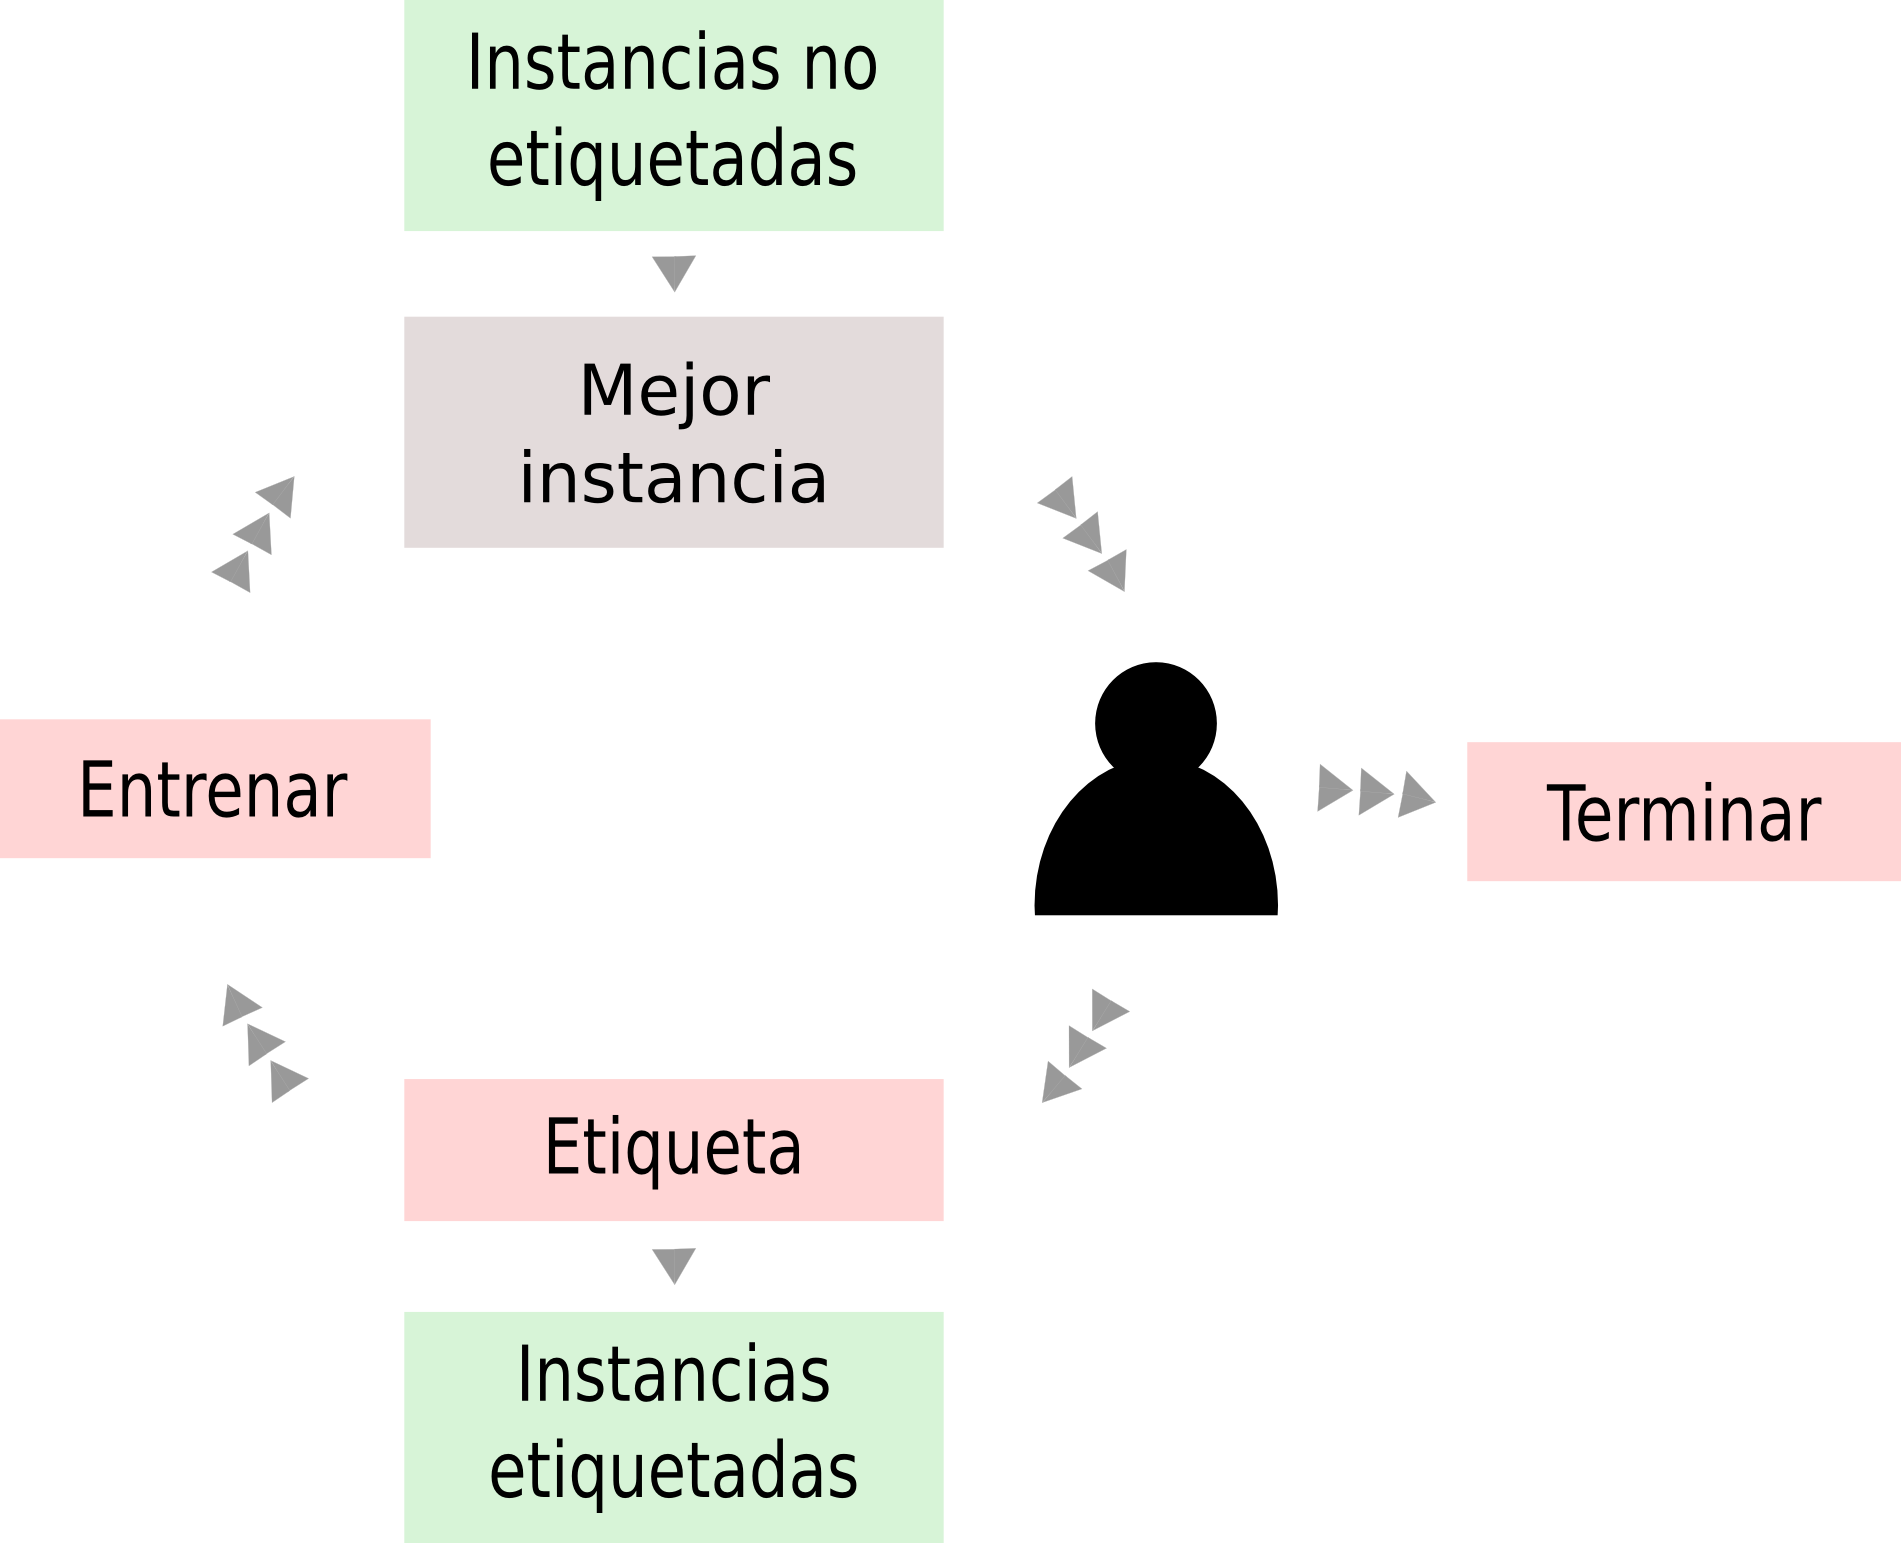
\includegraphics[width=8cm]{cicloaa.png}
\centering
\end{figure}

\citet{settles_active_learning_survey} explica que el aprendizaje activo es un paradigma donde el aprendedor selecciona preguntas para que un humano u oráculo las etiquete. La interacción aproximada entre el sistema y el oráculo se muestra en la figura \ref{cicloaa}. Si el aprendedor elige las instancias de las cuales puede aprender más información, entonces se minimiza la cantidad de instancias etiquetadas necesarias para lograr el mismo desempeño. La mayor motivación para este tipo de estrategias es la dificultad de conseguir datos etiquetados al mismo tiempo que se disponen de grandes cantidad de ejemplos no etiquetados, tal y como es nuestro caso. Utilizaremos, entonces, aprendizaje activo para entrenar el clasificador con la menor cantidad de consultas posibles a un usuario.

\subsection{Aprendizaje activo sobre características}

Durante las primeras etapas de desarrollo y especificación del problema debimos definir la representación de las instancias ante el clasificador. Sin embargo, al no existir trabajos previos con la misma proximación al problema no tenemos un punto de referencia para tomar como ejemplo. Por esto, decidimos incluir características tentativamente y realizar experimentos con aprendizaje activos sobre características e instancias.

%nos ayuda a entender mejor

En un enfoque como este se pedirá al usuario que etiquete las características seleccionadas con una clase si la presencia de la característica en una instancia es indicativa de la clase. \citet{settles-al-features} han realizado experimentos sobre clasificación de texto en donde se demuestra que el aprendizaje activo sobre características puede dar mejores resultados incluso que el aprendizaje sobre instancias. Durante este trabajo nos ayudará a identificar las características que mejor describen las instancias para la clasificación descripta.

\begin{figure}[h!]\label{aa-features}
\caption{Arquitectura de un sistema de aprendizaje activo sobre intancias y características.}
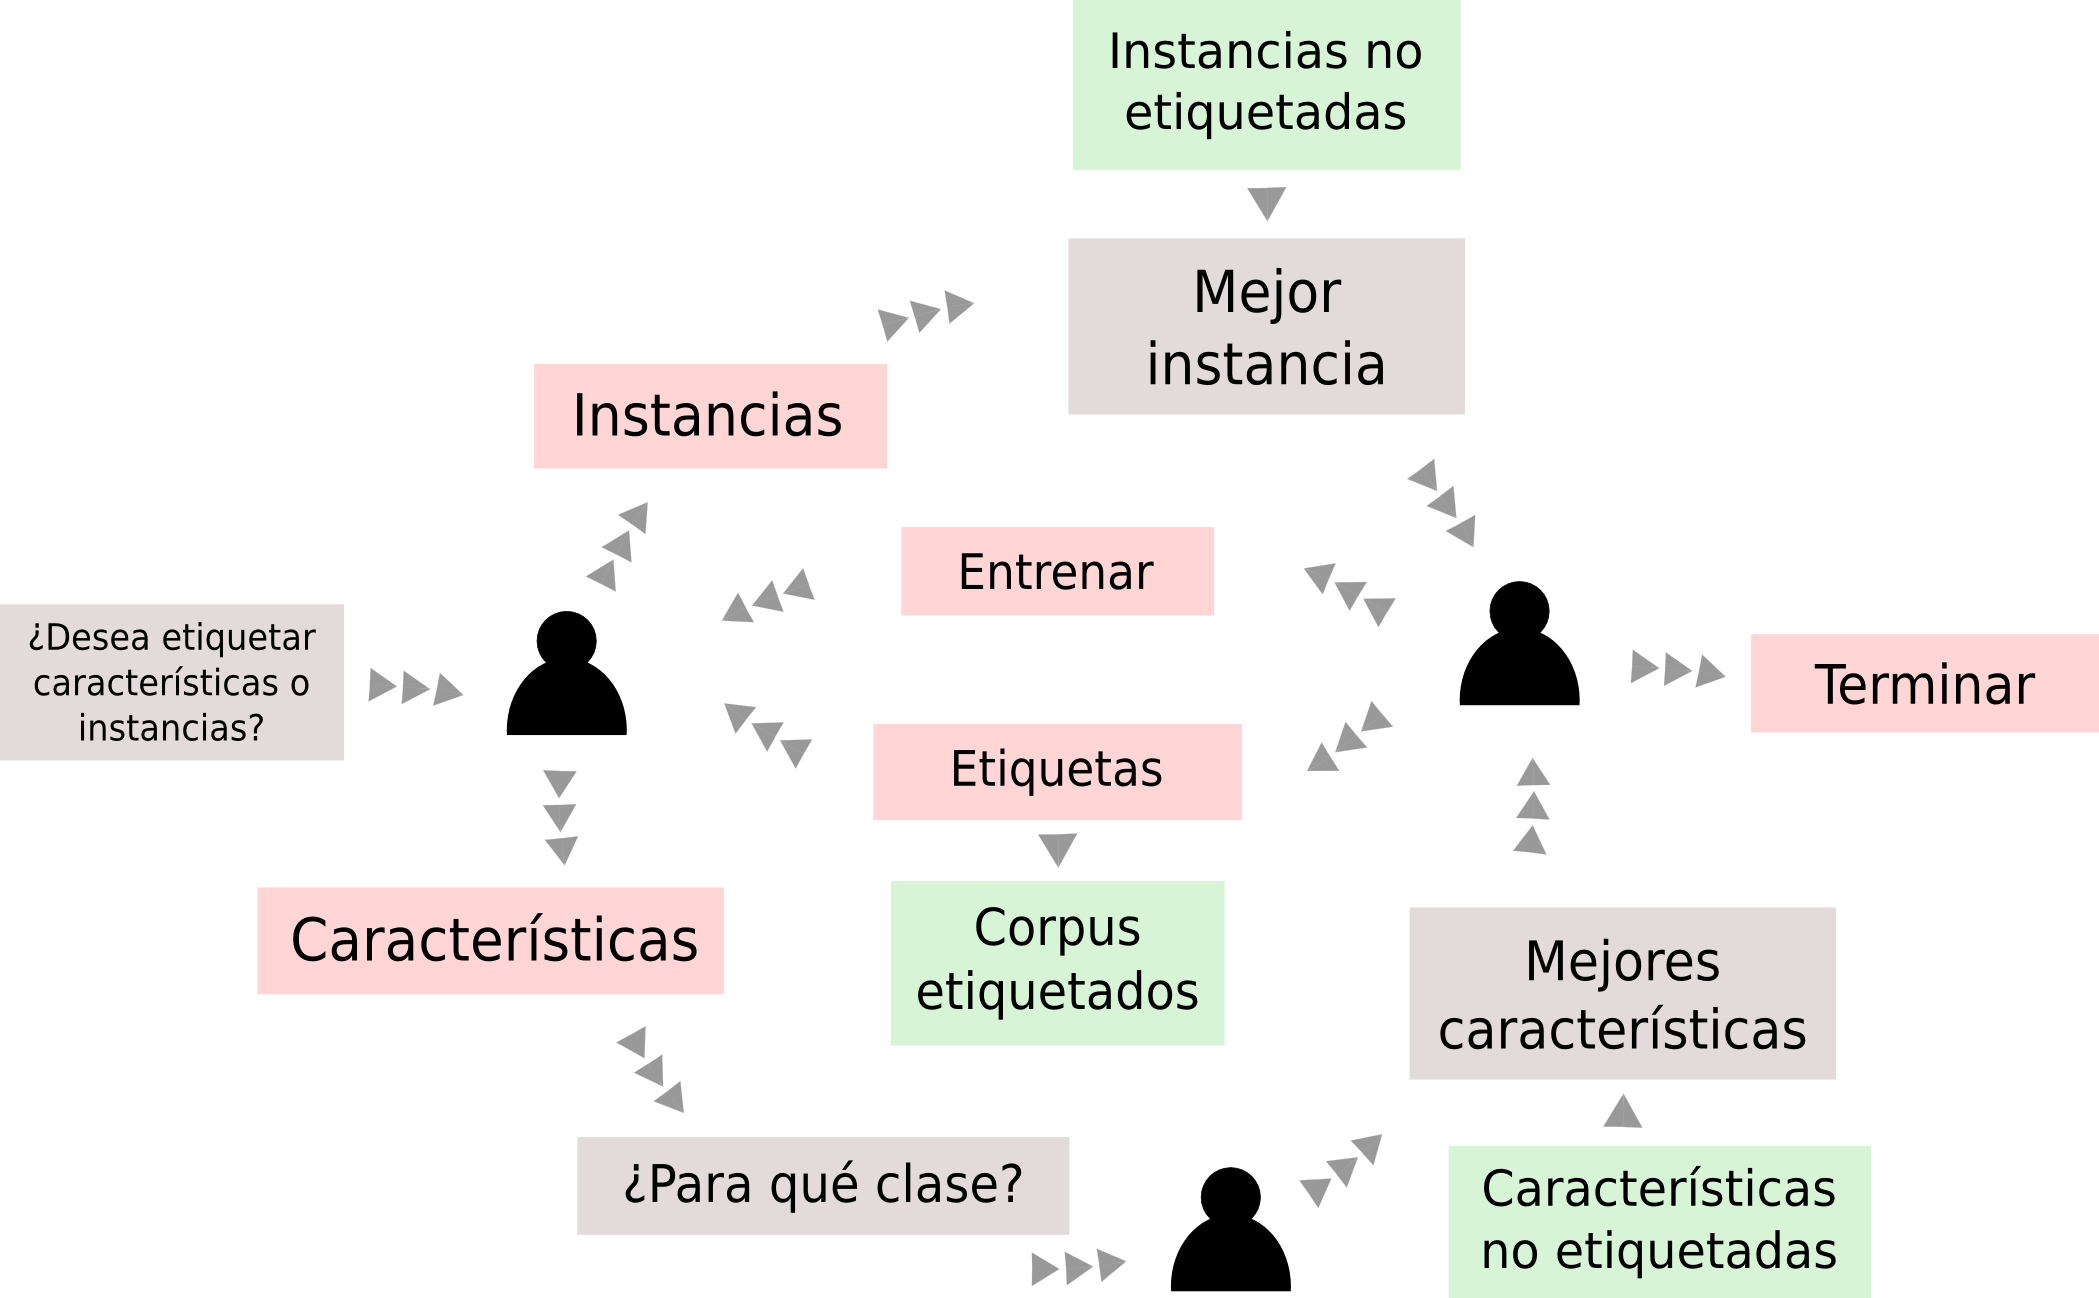
\includegraphics[width=12cm]{cicloaa-features}
\centering
\end{figure}

Las etiquetas obtenidas se utilizarán también para entrenar el clasificador reforzando la probabilidad de una característica dada una clase, como veremos en detalle en la implementación.

El usuario también tendrá la posibilidad de entrenar el clasificador con las etiquetas que ya ha ingresado o de terminar la sesión en cualquier momento. El diagrama de iteracción queda configurado como se muestra en la imagen \ref{aa-features}.

\begin{figure}[h!]\label{aa-features}
\caption{Arquitectura de un sistema de aprendizaje activo sobre intancias y características.}
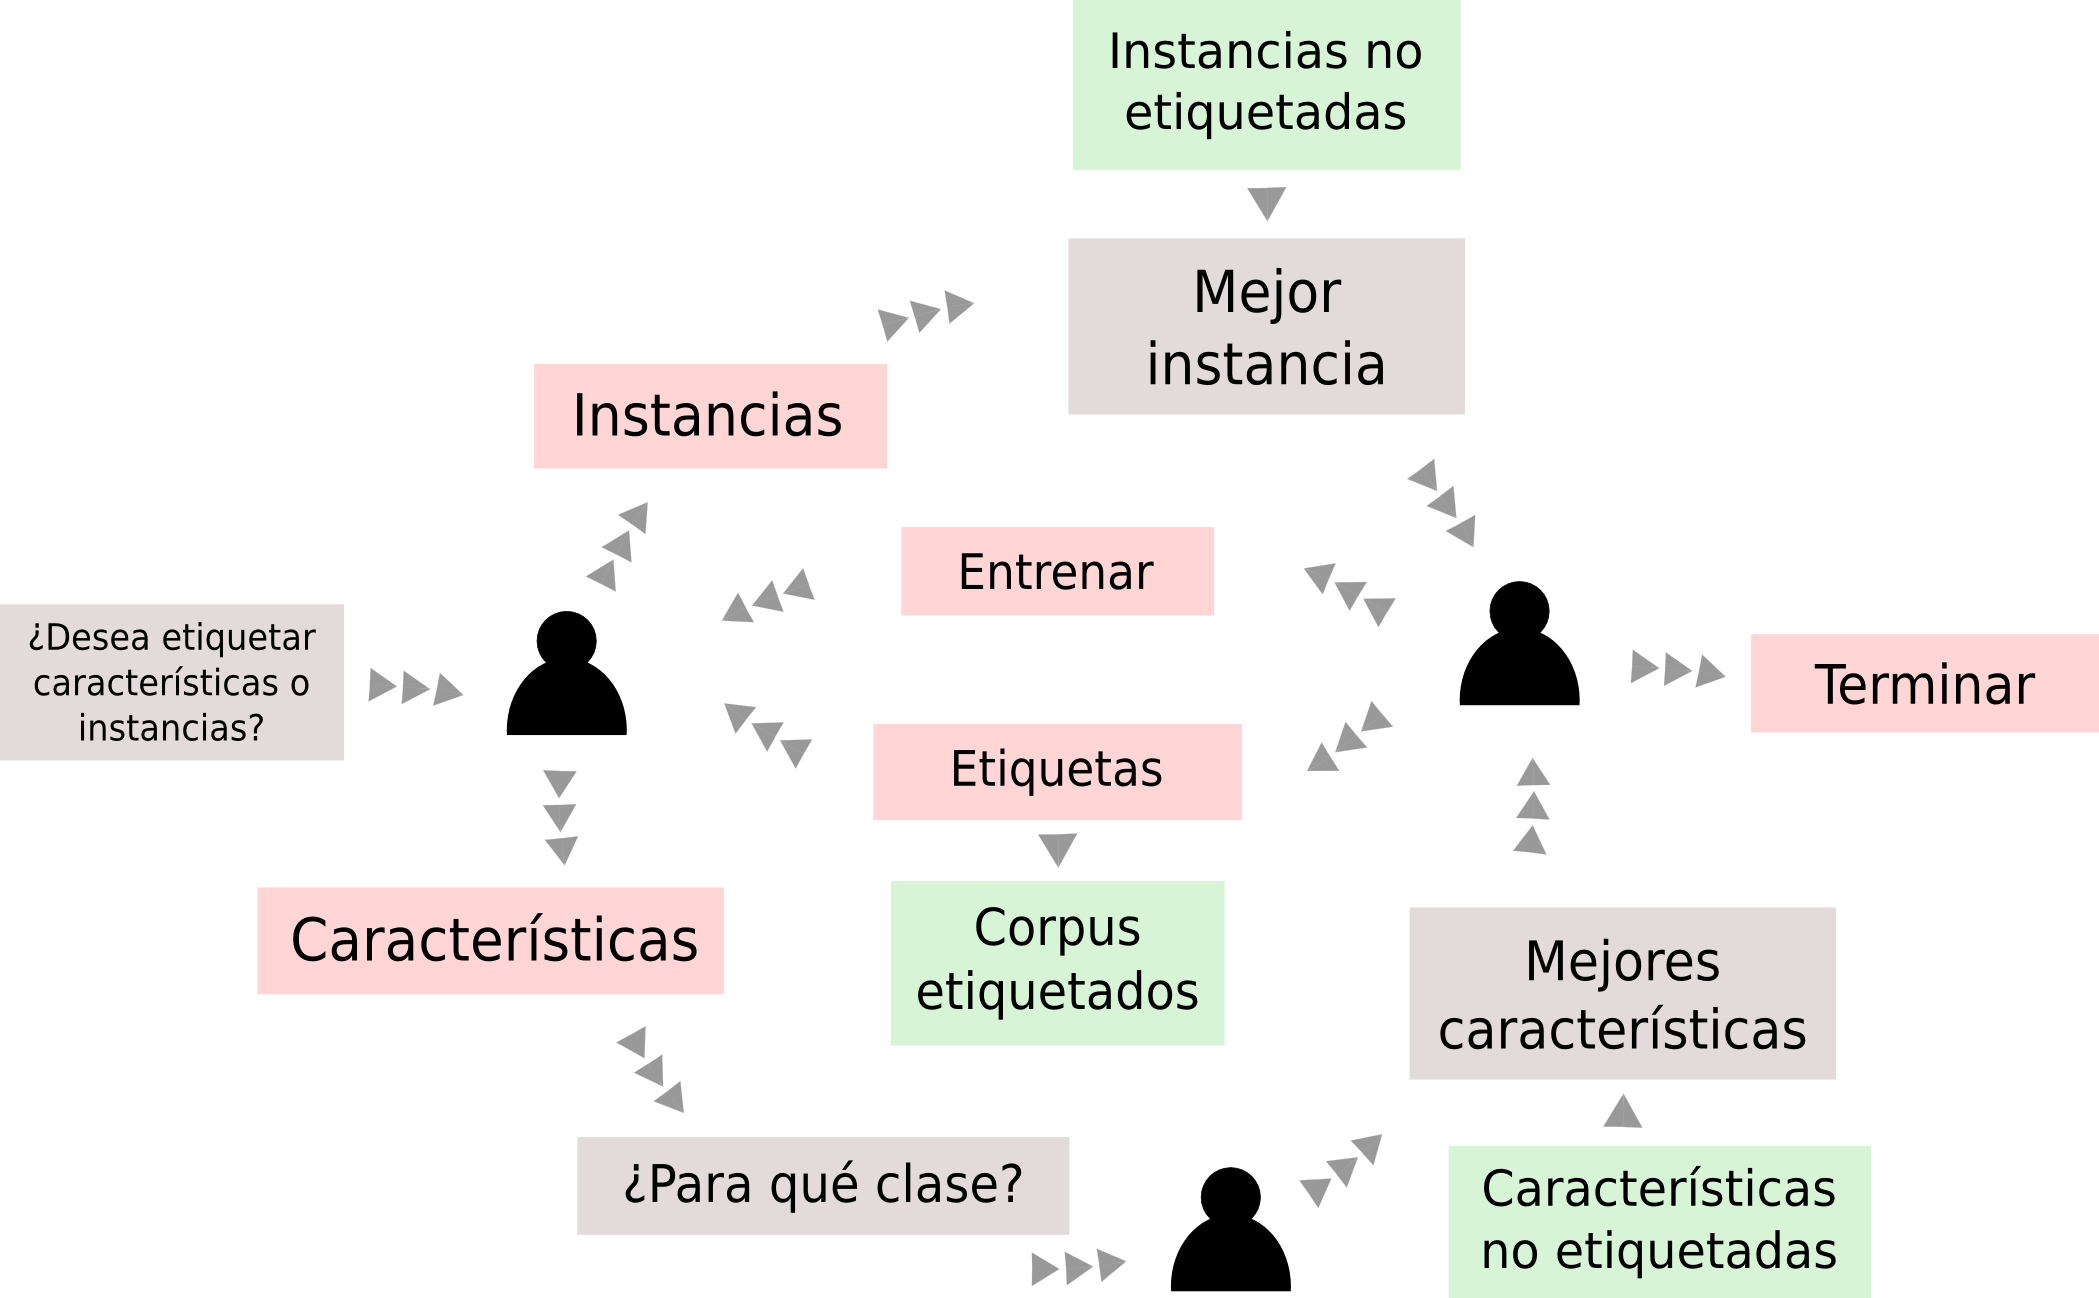
\includegraphics[width=12cm]{cicloaa-features}
\centering
\end{figure}

\subsection{Dualist}

Dualist es un sistema muy similar al que estamos planteando desarrollado por \citet{dualist} que combina el aprendizaje sobre instancias y sobre características. Los resultados presentados son para diversas tareas como el análisis de sentimientos o la clasificación de documentos.

\begin{figure}[h!]
\caption{Captura de pantalla de la interfáz gráfica de Dualist.}
\includegraphics[width=12cm]{dualist-screen}
\centering
\end{figure}

La interfaz gráfica de una instancia de Dualist se muestra en la figura \ref{figura-dualist} tiene dos secciones principales. A la izquierda se muestra una lista de instancias con las clases para que el usuario pueda etiquetarlas sólo con un click. A la derecha, por cada clase hay una lista de objetos seleccionables representando las características (en este caso palabras) que están potencialmente asociadas a la clase. \citet{dualist} sostienen que presentar al usuario toda la información en conjunto hará que éste etiquete una mayor cantidad antes de esperar a que el clasificador de reentrene o le presente nuevas opciones.

Nuestra implementación seguirá los mismos lineamientos principales que dualist: decidimos tomarlo como modelo ya que se centra en la interacción con el usuario y en la capacidad del software de ser utilizado en tiempo real. Nosotros deseamos lograr un sistema que sea viable de integrar con Quepy y complementar aplicaciones reales, en lugar de ser utilizado sólo para demostrar los resultados de este trabajo.


\chapter{Representación de las preguntas}\label{capitulo-features}

Una importante parte de cualquier problema que aborde el lenguaje natural es la forma de representarlo. Las características relevantes para describir un problema dependen fuertemente del mismo y de su solución, si bien existen numerosos ejemplos de trabajos previos a tomar como modelo. El siguiente paso es identificar qué características de la pregunta son indicativas de su clase semántica, lo cual no tiene una respuesta intuitiva.

Nuestra primera aproximación fue utilizar criterios estándares en la categorización de texto como los lemas de las palabras y sus etiquetas POS. \citet{Sebastiani-text-categorization} describe que a pesar de su simpleza son representaciones muy poderosas y que otras más complejas no necesariamente llevarán a un mejor desempeño del clasificador. A pesar de ser formas superficiales del lenguaje, son una manifestación de la semántica ya que ésta es su causa latente.

Además de lemas es común el uso de n-gramas para la representación de texto. Un n-grama es una secuencia de lemas de longitud n extraída del texto. Ilustramos este concepto con un ejemplo:

\begin{example} Descomposición de una oración en bigramas y trigramas.

Oración: ``El gato come pescado.''

Lemas: ``el'', ``gato'', ``comer'', ``pescado'', ``.''.

Bigramas: ``el gato'', ``gato comer'', ``comer pescado'', ``pescado .''.

Trigramas: ``el gato comer'', ``gato comer pescado'', ``comer pescado .''.

\end{example}

Se espera que los n-gramas representen además de las palabras del texto la relación que existe entre ellas derivada de su posición relativa. Sin embargo, estas combinaciones crecen exponencialmente con el tamaño del corpus y dan lugar a matrices muy esparsas, ya que pocos n-gramas ocurren en muchas instancias del corpus. Por ello decidimos limitarnos a bigramas y trigramas.

Los n-gramas pueden construirse no sólo a partir de los lemas sino también incluyendo etiquetas POS. Este tipo de estructuras son útiles cuando queremos representar, por ejemplo, ``la palabra comer seguida de un sustantivo''. Utilizaremos bigramas combinados de la forma (lema, POS) y (POS, lema), a las que llamamos bigramas mezclados.

\section{Subpatrones}

Como presentamos en el ejemplo \ref{preguntas-similares} algunas preguntas tienen tanto lemas como etiquetas POS muy similares y sin embargo pertenecen a clases distintas. La forma en la que Quepy distingue estos casos es utilizando la estructura de la frase, representada en sus patrones. Por eso, decidimos utilizar además como característica los patrones que concuerdan con la pregunta (\textit{pattern matching}).

Esta representación por sí sola tampoco mejora nuestra situación inicial, ya que sólo reconoce las preguntas que corresponden de forma exacta a un patrón. La solución que encontramos para este problema fue dividir cada patrón en todos sus posibles subpatrones y determinar con cuales de todos estos subpatrones concuerda cada instancia.

\begin{example} Subpatrones del ejemplo \ref{regex}.
\begin{enumerate}
\item \begin{lstlisting}
Lemma("what") + Lemma("be") + Question(Pos("DT"))
    + Group(Pos("NN"), "target") + Question(Pos("."))
\end{lstlisting}

\item
\begin{lstlisting}
Lemma("what") + Lemma("be") + Question(Pos("DT"))
+ Group(Pos("NN"), "target")
\end{lstlisting}

\item
\begin{lstlisting}
Lemma("what") + Lemma("be") + Question(Pos("DT"))
\end{lstlisting}

\item
\begin{lstlisting}
Lemma("what") + Lemma("be")
\end{lstlisting}

\item
\begin{lstlisting}
Lemma("what")
\end{lstlisting}

\item
\begin{lstlisting}
Lemma("be")
\end{lstlisting}

\item
\begin{lstlisting}
Lemma("be") + Question(Pos("DT"))
+ Group(Pos("NN"), "target") + Question(Pos("."))
\end{lstlisting}

\item
\begin{lstlisting}
...
\end{lstlisting}
\end{enumerate}
\end{example}

%La aplicación de Quepy original contaba con 29 patrones a partir de los cuales generamos 153 patrones parciales. De nuestro corpus original, sólo 56 pregun

\section{Nombres y tipos de entidades}

Existe un tipo más de característica que determina fuertemente la semántica de la pregunta. Recordemos que las ontologías son creadas colaborativamente por muchos usuarios que agregan porciones de datos e incluso definen el esquema de los mismos. Como resultado, la forma de acceder a una propiedad de una entidad dentro de la ontología está íntimamente ligada a la estructura que le dio el usuario al ingresar los datos. La misma propiedad como ``fecha de creación'' puede tener dos nombres distintos si nos referimos a entidades de tipo libro o de tipo película, llevando a la generación de consultas distintas. Por eso, en la situación que hemos propuesto, son necesarias dos clases semánticas en lugar de una, ya que las clases semánticas sirven de mediadoras entre la semántica y la ontología.

\begin{example} Ejemplos con semántica diferenciada por el tipo de la entidad.
    \begin{enumerate}
        \item ``Who are the actors of Titanic?''
        \item ``Who are the actors of Friends?''
    \end{enumerate}
En FreeBase, para obtener los actores que trabajaron en una película, como en el caso de la primera pregunta, debe utilizarse la relación ``/film/film/starring'', mientras que en el caso de una serie televisiva se utiliza ``/tv/tv\_program/regular\_cast''.
\end{example}

El indicio más certero de la clase semántica en estos casos es la entidad nombrada en la pregunta. Por ello, la incluimos como una característica más. Agregaremos los tipos de dicha entidad en la base de conocimiento, particularmente para esta aplicación FreeBase. Cabe destacar que no todas las preguntas tienen una entidad, y en el caso de que sí tenga no siempre podemos reconocerla. Esto depende del sistema externo de reconocimiento de nombres de entidades o NER por sus siglas en inglés. En el capítulo siguiente describiremos el sistema que utilizamos para esta tarea.

En resumen, las características propuestas para el sistema son:
\begin{itemize}
    \item Etiquetas POS.
    \item Lemas, bigramas, trigramas y bigramas mezclados.
    \item Concordancias a patrones parciales.
    \item Entidad nombrada.
    \item Tipos de la entidad nombrada.
\end{itemize}


\chapter{Implementación}

\section{Arquitectura del sistema}
Si bien el objetivo principal de este trabajo es incrementar la cobertura de Quepy, deseamos también que el sistema esté compartimentado de tal forma que sus componentes puedan utilizarse individualmente para otras aplicaciones.

La arquitectura de nuestro sistema integra tres grandes bloques que interactúan a través de interfaces:

\begin{description}
    \item[FeatMultinomialNB] Es el clasificador del sistema. Hereda del clasificador multinomial bayesiano \textit{MultinomialNB} de la librería scikit-learn desarrollada por \citet{scikit-learn} y está adaptado para soportar el entrenamiento utilizando tanto instancias como características. Agregamos algunos métodos auxiliares más a la clase que simplifican algunos cálculos para el aprendizaje activo.
    \item[ActivePipeline] Es una clase que abstrae los ciclos de aprendizaje activo. Recordemos que constan de dos pasos principales donde se seleccionan las instancias (o características) y luego se procesan las etiqueta devueltas por el usuario. Para llevar a cabo estas tareas el pipe necesita tener acceso a los corpus etiquetados y no etiquetados y al clasificador, lo cual lo convierte en el módulo central del proyecto.
    \item[Preprocess] Es un módulo que convierte las preguntas de entrenamiento etiquetadas a su representación matricial utilizando las características descriptas en el capítulo anterior. La representación de las preguntas está completamente ligada a los patrones de la aplicación de Quepy. Por ello diseñamos el preproceso como una extensión opcional de Quepy que puede utilizar cualquier clasificador. En otras palabras, no es necesario que se integre con aprendizaje activo.
\end{description}

\subsection{ActivePipeline: Un marco de trabajo de aprendizaje activo sobre características e instancias}

ActivePipeline es una clase creada para simplificar la tarea del aprendizaje activo. Entre las actividades que realiza se encuentra la lectura de los corpus, la selección de instancias y características para presentar al usuario, la gestión de los datos ingresados y el reentrenamiento del clasificador. También agregamos funciones que no eran necesarias pero facilitan el entorno de experimentación como sessiones y métricas de evaluación parcial.

Hasta el momento hemos realizado la prueba de concepto que demuestra que una aproximación de este estilo ayudaría a resolver el problema de la falta de cobertura de Quepy. Esta arquitectura está en desarrollo constante y no ha sido pulida para interactuar con un sistema real. Describiremos a continuación los puntos más centrales de la implementación ya que los detalles son altamente propensos a ser modificados en el futuro.

Para crear una instancia de ActivePipeline se requiere un diccionario con los siguientes parámetros:
\begin{description}
    \item[Clasificador] Es una instancia de un clasificador. Para mantener generalidad, requerimos que tenga la interfaz estándar de sklearn. Los métodos que utilizamos son \textit{fit}, \textit{predict\_proba}, \textit{predict\_log\_proba} y \textit{score}.
    \item[Corpus] Se deben definir los archivos desde donde recuperar al menos tres corpus: el de entrenamiento, el de evaluación y el no etiquetado. Los corpus ya deben estar procesados antes de ser leídos por el ActivePipeline, y es recomendable que sean instancias de una clase Corpus también definida en el sistema.
\end{description}
Al permitir elegir tanto características como el corpus y el clasificador, la clase ActivePipeline puede ser utilizada dentro de cualquier ámbito incluso no relacionado al procesamiento del lenguaje natural.

Tanto para el aprendizaje sobre características y sobre instancias el ActivePipeline cuenta con una función automática. El usuario debe definir sólo las funciones de interacción con el usuario, es decir, cómo mostrar la información, y pasarlas como parámetros al ActivePipeline.

\subsection{FeatMultinomialNB: Un clasificador entrenado con características}

Como ya mencionamos anteriormente FeatMultinomialNB es un clasificador bayesiano ingenuo. Profundizaremos ahora en el fundamente teórico detrás de él y en las modificaciones que realizamos para soportar el entrenamiento con características.

Un clasificador bayesiano, explica \citet{libro-abney}, es un ejemplo de un modelo generativo. Estos modelos usualmente utilizan la distribución anterior de las clases $P(c)$ y la distribución de las instancias específica para la clase o verosimilitud $P(x|y)$. Su nombre se debe a que un modelo es una hipótesis acerca de cómo cada instancia puede ser generada por una clase. Se utiliza esta probabilidad generativa para la clasificación a través del teorema de Bayes:

$$P(x|c) = \frac{P(c)P(x|y)}{P(x)}$$

El \textit{MultinomialNB} descripto por \citet{multinomial-manning} se basa en la asunción ingenua de que el valor de cada una de las características de una instancia es independiente de las demás. Si bien sabemos que esto no es así y que cada característica sí se relaciona con las restantes, este clasficador ampliamente utilizado para la categorización de texto \citet{dualist}, \citet{multinomialnb-comparision-mccallum} y \citet{multinomialnb-unbalanced}. Su principal ventaja es la simplicidad, lo que en nuestro caso ayudó en la tarea de la modificación.

En gran parte de la bibliografía se asume que las características de una instancia serán sólo las palabras presentes en el documento o instancia, lo cual no se ajusta a la representación elegida para este problema. Por lo tanto, hemos cambiado levemente la notación que utilizan otros autores reemplazando palabras como \textit{words} o \textit{terms} por \textit{características}. También hemos reemplazado \textit{documents} por \textit{instancias}.

Bajo este modelo, la probabilidad de que una instancia $x_i$ sea de clase $c_j$ es computada utilizando la fórmula:
\begin{equation}\label{eq-mnb-prob}
    P(c_j|x_i) \propto P(c_j) \prod_{1\leq k \leq n_i}P(f_k|c_j)
\end{equation}
donde $n_i$ es la cantidad de características que aparecen en la instancia $x_i$ y $P(f_k|c_j)$ es la probabilidad de que la característica $f_k$ esté presente en una instancia de clase $c_j$. \citet{multinomial-manning} explican que la intuición detrás de estos conceptos es que $P(f_k|c_j)$ indica de qué tan buen indicador es $f_k$ para la clase $c_j$, mientras que $P(c_j)$ pesa estos valores por la probabilidad de la clase. El producto de las probabilidades y pesos es una medida de cuánta evidencia existe de que la instancia pertenezca a la clase.

La gran cantidad de multiplicaciones sobre probabilidades menores que uno puede llevar fácilmente a un desbordamiento aritmético debido la imposibilidad de representar números tan pequeños en una computadora. Utilizaremos logaritmos para manejar esta situación, manteniendo la proporción de los operandos ya que el logaritmo es una función monótona creciente y basándonos fuertemente en la propiedad que asegura $\log(ab) = \log(a) + \log(b)$. La ecuación \ref{eq-mnb-prob} es equivalente a:

\begin{equation}
\log P(c_j|x_i) \propto \log P(c_j) + \sum_{1\leq k \leq n_i} \log P(f_k|c_j)
\end{equation}

La tarea de clasificación se reduce entonces a encontrar la clase $c_j$ que maximice la ecuación \ref{eq-mnb-prob}. Volviendo a la definición \ref{def-clasificacion}, podemos reescribirla como:

\begin{definition}
\begin{equation}
    \Phi(x_i) = \operatorname*{argmax}_{c_j \, \in \, \mathcal{C}} \; \log P(c_j|x_i) = \operatorname*{argmax}_{c_j \, \in \, \mathcal{C}} \; \log P(c_j) + \sum_{1\leq k \leq n_i} \log P(f_k|c_j)
\end{equation}
\end{definition}

Nuestro modelos depende entonces de dos parámetros: $P(c_j)$ y $P(f_k|c_j)$. Sin embargo no conocemos las distribuciones reales de estas variables, y por lo tanto las estimaremos empíricamente a partir de los datos observados. Llamaremos $\hat{P}(c_j)$ y $\hat{P}(f_k|c_j)$ a las estimaciones respectivamente, que se calculan utilizando estimadores de máxima verosimilitud:

\begin{equation}
\hat{P}(c_j) = \frac{\sum_{x \in \mathcal{L}} \, \hat{\Psi}(x, c_j)}{|\mathcal{L}|}
\end{equation}
\begin{equation}\label{sin-smooth}
\hat{P}(f_k|c_j) = \frac{\sum_{x \in \mathcal{L}} \, \hat{\Psi}(x, c_j) f_k(x)}{\sum_{x \in \mathcal{L}} \, f_k(x)}
\end{equation}

donde $\mathcal{L}$ es el conjunto de datos etiquetados de entrenamiento, $\hat{\Psi}(x, c_j) \in \{0,1\}$ es el clasificación obtenida del mismo y $f_k(x)$ es la cantidad de veces que la característica $f_k$ está presente en la instancia $x$.

Aunque las ecuaciones están bien definidas, puede suceder que el numerador de la ecuación \ref{sin-smooth} $\sum_{x \in \mathcal{L}} \hat{\Psi}(x, c_j) f_k(x)$ sea nulo ya que una característica puede no ocurrir en ninguna instancia de la clase. Debido a la raleza en la distribución de palabras explicada por \citet{zipf1}, \citet{zipf2}, es común que ocurra este fenómeno. Para evitarlo se suaviza los datos de la siguiente manera:

\begin{equation}
\hat{P}(f_k|c_j) = \frac{m_{jk} + \sum_{x \in \mathcal{L}} \hat{\Psi}(x, c_j) f_k(x)}{\sum_{x \in \mathcal{L}} (f_k(x) + m_k)}
\end{equation}

\citet{dualist} plantea que $m_{jk}$ es la probabilidad anterior de $f_k$ para la clase $c_j$, y comunmente se utiliza una distribución uniforme como la Laplaciana donde todos los valores son 1. El término $m_k$ es un valor para normalizar la división.

Nuestro objetivo principal es adaptar este clasificador para que utilize un parámetro adicional $m_{jk}$ modificando esta probabilidad anterior en base a las etiquetas del usuario para las características. Introduciremos entonces la siguiente definición:

\begin{definition}
La clasificación de una características es una función $\Psi_f:\mathcal{F} \times \mathcal{C} \rightarrow \{0, 1\}$ que asigna valores booleanos donde $\mathcal{F}$ es el conjunto de características y $\mathcal{C}$ es el conjunto de clases posibles.
\end{definition}

Seguimos la implementación de dualist para agregar esta clasificación adicional de la siguiente manera:

\begin{equation}\label{eq-feat-boost}
m_{jk} = 1 + \Psi_f(f_k, c_j) \; \alpha
\end{equation}

donde $\alpha$ es una constante y $\Psi_f$ es la clasificación aprendida del usuario.


\section{Selección de instancias}

Elegir las instancias para que sean etiquetadas por el usuario es el centro de los algoritmos de aprendizaje activo y existen numerosas estrategias que pueden utilizarse. Trabajos como \citet{settles_active_learning_survey} y \citet{al-logistic-regresion-schein} resumen las más importantes de ellas:

\begin{description}
    \item[Muestro por incertidumbre] Asumiendo que el aprendedor tiene cierto
    grado de certidumbre a la hora de etiquetar un ejemplo, hay varias formas
    de utilizar esta información para seleccionar los ejemplos que se enviarán
    al oráculo:
    \begin{itemize}
        \item Confianza o incertidumbre en su clasificación.
        \item Distancia entre la dos primeras etiquetas más probables.
        \item Entropía.
    \end{itemize}
    Estudios han demostrado que dichas estrategias obtienen resultados similares
    y que la elección debe hacerse teniendo en cuenta la aplicación particular
    para la que se utilizarán.
    \item[Selección por comité (QBC)] Se utilizan varios clasificadores para obtener
    un conjunto de etiquetas para cada una de las instancias no etiquetadas.
    Luego se seleccionan las instancias que hayan generado mayor desacuerdo
    entre los clasificadores.
    \item[Cambio esperado del modelo] Selecciona las instancias que generarían
    un mayor cambio en el modelo (aprendedor) si se supiera su etiqueta. Como
    medida de cambio se utiliza el largo del gradiente del modelo (EGL). Se ha
    demostrado que funciona bien empíricamente, pero puede ser
    computacionalmente caro.
    \item[Reducción del error esperado] Es similar al método anterior, pero en
    lugar de maximizar el cambio en el modelo, minimiza su error de
    generalización. El objetivo es reducir el número esperado de predicciones
    erróneas. Este método ha sido ampliamente estudiado demostrando muy buenos
    resultados, sin embargo, es el método computacionalmente más costoso.
    \item[Reducción de la varianza] Intenta minimizar el error esperado
    indirectamente minimizando la varianza de los resultados. Para ello,
    selecciona un conjunto de instancias que maximice la información Fisher. Al
    igual que en el método anterior se tiene en cuenta todo es espacio de
    ejemplos en lugar de cada una de las instancias, y por lo tanto tiene menos
    probabilidades de seleccionar ejemplos raros en la distribución.
    \item[Métodos pesados por la densidad] Siguiendo la misma línea que los dos
    métodos anteriores, supone que los ejemplos significativos son aquellos
    que no solo tienen alta incertidumbre, sino que son representativos
    de la distribución subyacente. Estudios indican resultados superiores,
    acompañados por implementaciones de alta velocidad que permiten incluso
    interacción de tiempo real con el usuario.
\end{description}

De todas estas opciones elegimos explorar el espacio de instancias a través de la entropía definida por \citet{entropy-shannon} como:
\begin{equation*}
\mathcal{H}(x) = - \sum_{c_i\,\in\,\mathcal{C}} \, P(c_i|x)\; \log\,P(c_i|x)
\end{equation*}
\citet{information-theory-cover} explica en términos simples que la entropía es la cantidad de información necesaria para representar una variable aleatoria. \citet{multinomial-manning} plantea también que la entropía es una forma de medir la incertumbre, ya que se maximiza cuando las etiquetas para una instancia son equiprobales y se vuelve 0 cuando la instacia está etiquetada.

Este método ha sido utilizado previamente como parte del aprendizaje activo por \citet{entropy-or}, \citet{settles-entropy} y \citet{Hwa-entropy}. Nosotros lo tomamos por varios motivos:
\begin{itemize}
    \item Es simple y rápido de calcular.
    \item Tiene en cuenta la incertidumbre de todas las clases, no solo una o dos de ellas.
    \item \citet{settles_active_learning_survey} sostiene que la entropía es más adecuada cuando se busca minimizar la pérdida o \textit{log-loss}, definida como la desviación de la clasificación; mientras que los otros métodos son adecuados para minimizar el error. En particular buscamos que el clasificador se desempeñe correctamente en todas las clases y no solo en la clase mayoritaria.
\end{itemize}


% In the case of uncertainty sampling using the Shannon entropy measure of uncertainty, bad performance goes hand by hand with noise, as defined by the portion of squared error that is training set size independent. For margin sampling, inability to identify the pairs of categories forming the margin on multi-category problems is the biggest danger, as seen on the NewsGroups data set. In spite of this observation, margin sampling competes favorably with the alternative heurstics and is the most computationally efficient method examined.

\section{Selección de características}\label{instance-selection}

Un criterio ampliamente utilizado para la selección de características es la Ganancia de Información o \textit{Information Gain}. Algunos estudios que destacan su uso como medida de relevancia son \citet{dualist}, \citet{forman-ig} y \citet{Sebastiani-text-categorization}

\citet{infgain} define la ganancia de información como la cantidad de información en bits sobre la predicción de la clase, si la única información disponible es la presencia de la característica y la distribución de la clase correspondiente. En otras palabras, mide la reducción esperada de la entropía cuando la característica está presente o ausente. Podemos expresarla según la siguiente fórmula:

\begin{equation}
\mathcal{IG}(\mathcal{X}, \mathcal{Y}) = \mathcal{H}(\mathcal{X}) - \mathcal{H}(\mathcal{X}|\mathcal{Y}) = \mathcal{H}(\mathcal{Y}) - \mathcal{H}(\mathcal{Y}|\mathcal{X})
\end{equation}

Notemos que es una función entre variables aleatorias, donde una es la presencia de una característica y otra es la clase. Para la clasificación de texto en particular, podemos reemplazar la fórmula de la entropía y definir la ganancia de información como:

\begin{equation}
\mathcal{IG}(f_k) = \sum_{I_k} \sum_j P(I_k, c_j)\,\log \frac{P(I_k,c_j)}{P(I_k)P(c_j)}
\end{equation}

donde $I_k \in \{0, 1\}$ indica la presencia o ausencia de la característica k.

Algunas de estas probabilidades no son parte de nuestro, por lo que las estimamos empíricamente como:
$$ \hat{P}(I_k = 1) = \frac{|\{ x \in \mathcal{X}: f_k(x) > 0 \} |}{|\mathcal{X}|} $$
$$ \hat{P}(I_k = z, c_j) = \frac{|\{ x \in \mathcal{X}: I_k(x) = z \wedge \Psi(x, c_j)\} |}{|\mathcal{X}|} $$
$$ \hat{P}(I_k = 0) = 1 - \hat{P}(I_k = 1) $$
donde $\mathcal{X}$ es el conjunto de instancias.

Para simplificar la tarea de etiquetamiento, presentamos al usuario las características asociadas a las clases para las que son más probables. Esta selección se realiza en dos pasos: primero seleccionamos las k características que coocurren más veces con la clase y luego las ordenamos por su ganancia de información.

\section{Maximización de la esperanza}
El algoritmo de maximización de la esperanza propuesto por \citet{Dempster-maximumlikelihood} es ampliamente utilizado para inferir parámetros desconocidos en una distribución que tiene estados latentes. Si conocieramos el universo completo de instancias posibles y sus clases correspondientes, entonces podríamos estimar los parámetros de un clasificador directamente utilizando máxima verosimilitud. Sin embargo, no conocemos parte de este universo, lo cual constituye nuestros estados latentes.

Ya hemos definido previamente el concepto de verosimilitud o \textit{likelihood} del modelo: es una función sobre los parámetros del modelo y un conjunto de datos que calcula la probabilidad de los valores tomados por cada variable aleatoria del modelo bajo dichos parámetros. Podemos escribirlo como:

\begin{equation}
L(\theta) = P(\mathcal{X}_l, \mathcal{C}_l; \theta)
\end{equation}

donde $\theta$ representa a los parámetros y $\mathcal{L} = (\mathcal{X}_l, \mathcal{C}_l)$. Como las instancias de entrenamiento se asume que son i.i.d., entonces podemos escribir las dos siguientes fórmulas equivalentes:

\begin{equation}
L(\theta) = \prod_{x_i, c_i \in \mathcal{L}} P(x_i, c_i; \theta)
\end{equation}
\begin{equation}
l(\theta) = \log L(\theta) = \sum_{x_i, c_i \in \mathcal{L}} \log P(x_i, c_i; \theta)
\end{equation}

Si llamamos $cant(c_j)$ a la cantidad de instancias etiquetadas con la clase $c_j$, entonces definimos:

\begin{equation}
l(\theta) = \sum_{x_i \in \mathcal{L}, \, c_j \in \mathcal{C}} cant(c_j) \log P(x_i, c_j; \theta)
\end{equation}

\begin{equation}\label{loglikelihood}
l(\theta) = |\mathcal{X}_l| \sum_{x_i \in \mathcal{L}, \, c_j \in \mathcal{C}} P(c_j) \log P(x_i, c_j; \theta)
\end{equation}


A grandes rasgos, el algoritmo funciona en dos pasos E y M, por sus siglas en inglés \textit{Expectation} y \textit{Maximization}.

El paso E es el que calcula el valor esperado de la verosimilitud asumiendo que la distribución actual es verdadera y no existen variables no observadas. Para realizarlo, utilizamos el clasificador en su estado actual para etiquetar probabilisticamente el conjunto de datos no etiquetados, y asumimos dichas etiquetas como correctas. Con este conjunto de nuevos datos se calcula el $l(\theta)$ del modelo según la ecuación \ref{loglikelihood}.

Si los parámetros actuales fueran correctos, entonces la verosimilitud obtenida sería la verosimilitud real del modelo, pero como no lo son provee una cota inferior. Luego, como tenemos una función sin valores no observados, el paso M maximiza $l(\theta)$ encontrando parámetros del modelo más adecuados. De esta forma optimizamos la cota inferior encontrada generando un nuevo conjunto de parámetros $\hat{\theta}$.

Ambos pasos se repite numerosas veces hasta lograr convengercia. Sin embargo tomamos ejemplo de Settles y realizamos una sola iteración, dado que argumenta que las siguientes iteraciones no aportan significativamente a la precisión del clasificador.

Si bien derivar la maximización correcta de los parámetros del $FeatMultinomialNB$ no es trivial, la implementación posterior sí es sencilla. Para realizarlo nos basamos en la maximización de un clasificador Bayesiano simple de \citet{data-mining-Liu}, agregando la noción de \citet{dualist} de utilizar tanto los datos etiquetados como no etiquetados pesando los no etiquetados por un factor de 0,1.

Al etiquetar los ejemplos no anotados obtenemos una matriz con $P(c_j|x_i)$ para cada instancia y cada clase. Utilizamos esta matriz para reestimar los parámetros de la siguiente forma:

\begin{equation*}
\hat{P}_u(c_j) = \sum_{x_i \in \mathcal{U}} P(c_j|x_i) P(x_i)
\end{equation*}
\begin{equation*}
\hat{P}_u(f_k|c_j) = \sum_{x_i \in \mathcal{U}} P(c_j|x_i) P(x_i) f_k(x_i)
\end{equation*}

\begin{equation*}
\hat{P}_l(c_j) = \sum_{x_i \in \mathcal{U}} P(c_j|x_i) \Psi(x_i, c_j)
\end{equation*}
\begin{equation*}
\hat{P}_l(f_k|c_j) = \sum_{x_i \in \mathcal{U}} P(c_j|x_i) \Psi(x_i, c_j) f_k(x_i)
\end{equation*}

\begin{equation}
\hat{P}(c_j) = \frac{0.9 * \hat{P}_l(c_j) + 0.1 * \hat{P}_u(c_j)}{\mathcal{Z}_1}
\end{equation}
\begin{equation}
\hat{P}(f_k|c_j) = \frac{0.9 * \hat{P}_l(f_k|c_j) + 0.1 * \hat{P}_u(f_k|c_j)}{\mathcal{Z}_2}
\end{equation}

donde $\mathcal{U}$ es el conjunto de datos no etiquetados y $\mathcal{Z}_1$, $\mathcal{Z}_2$ son contantes de normalización.
%http://ai.stanford.edu/~chuongdo/papers/em_tutorial.pdf

% http://stackoverflow.com/questions/11808074/what-is-an-intuitive-explanation-of-expectation-maximization-technique

% http://cs.brown.edu/courses/cs195-5/fall2009/docs/lecture_11-12.pdf

% http://cs229.stanford.edu/notes/cs229-notes8.pdf


% Descripción de los corpus.
    % Etiquetado
        % Las semillas son muy importantes. Deberían ser elegidas al azar?
        % La muestra debería ser representativa de la población? Aproximadamente un 10% de las preguntas son reconocidas por quepy, deberíamos incluir esto en el set de entrenamiento?
    % No etiquetado
    % Testing
        % Las que reconoce quepy?
        % 500 preguntas está bien?


% Testing corpus: 31 recognized instances
% Testing corpus: 186 total instances
% Numbers of classes in Testing corpus  29
% Training corpus 19 recognized questions
% Training corpus total instances  29
% Unlabeled corpus 8 recognized instances
% Unlabeled corpus total instances  497
% booksbyauthor & 3 & 1 & 8 \\
% listmovies & 1 & 1 & 0 \\
% listtvshows & 1 & 1 & 1 \\
% howoldis & 5 & 1 & 14 \\
% movieduration & 1 & 1 & 1 \\
% presidentsof & 2 & 1 & 3 \\
% directorof & 1 & 1 & 0 \\
% populationof & 1 & 1 & 3 \\
% plotof & 1 & 1 & 2 \\
% whois & 1 & 1 & 0 \\
% whowrote & 1 & 1 & 0 \\
% castof & 1 & 1 & 3 \\
% whereis & 3 & 1 & 8 \\
% other & 135 & 1 & 404 \\
% moviereleasedate & 1 & 1 & 1 \\
% actorsof & 2 & 1 & 0 \\
% whereisfrom & 4 & 1 & 8 \\
% spokenlanguageof & 1 & 1 & 3 \\
% bandmembers & 2 & 1 & 5 \\
% showswith & 1 & 1 & 3 \\
% musicgenre & 1 & 1 & 3 \\
% capitalcityof & 1 & 1 & 1 \\
% albumsofband & 5 & 1 & 10 \\
% creatorof & 2 & 1 & 4 \\
% whatis & 1 & 1 & 2 \\
% episodecount & 1 & 1 & 0 \\
% actedon & 4 & 1 & 7 \\
% bandfoundation & 2 & 1 & 2 \\
% moviesbydirector & 1 & 1 & 1 \\

% Distribución actual del corpus:
% Quepy questions 115
%   Recognized 58
%   Unrecognized 57
% Other questions 6658
%   Labeled 607
%   Unlabeled 6051

% Test corpus 250
% Training corpus 165
% Unlabeled corpus 6358

% Testing corpus: 31 recognized instances
% Testing corpus: 186 total instances
% Numbers of classes in Testing corpus  29
% Training corpus 19 recognized questions
% Training corpus total instances  29
% Unlabeled corpus 8 recognized instances
% Unlabeled corpus total instances  115
% booksbyauthor & 3 & 1 & 8 \\
% listmovies & 1 & 1 & 0 \\
% listtvshows & 1 & 1 & 1 \\
% howoldis & 5 & 1 & 14 \\
% movieduration & 1 & 1 & 1 \\
% presidentsof & 2 & 1 & 3 \\
% directorof & 1 & 1 & 0 \\
% populationof & 1 & 1 & 3 \\
% plotof & 1 & 1 & 2 \\
% whois & 1 & 1 & 0 \\
% whowrote & 1 & 1 & 0 \\
% castof & 1 & 1 & 4 \\
% whereis & 3 & 1 & 8 \\
% other & 135 & 1 & 14 \\
% moviereleasedate & 1 & 1 & 1 \\
% actorsof & 2 & 1 & 1 \\
% whereisfrom & 4 & 1 & 8 \\
% spokenlanguageof & 1 & 1 & 3 \\
% bandmembers & 2 & 1 & 6 \\
% showswith & 1 & 1 & 4 \\
% musicgenre & 1 & 1 & 3 \\
% capitalcityof & 1 & 1 & 1 \\
% albumsofband & 5 & 1 & 11 \\
% creatorof & 2 & 1 & 4 \\
% whatis & 1 & 1 & 2 \\
% episodecount & 1 & 1 & 0 \\
% actedon & 4 & 1 & 9 \\
% bandfoundation & 2 & 1 & 2 \\
% moviesbydirector & 1 & 1 & 2 \\

% Testing corpus: 17 recognized instances
% Testing corpus: 172 total instances
% Numbers of classes in Testing corpus  16
% Training corpus 10 recognized questions
% Training corpus total instances  16
% Unlabeled corpus 6 recognized instances
% Unlabeled corpus total instances  104
% booksbyauthor & 3 & 1 & 8 \\
% creatorof & 2 & 1 & 4 \\
% bandfoundation & 2 & 1 & 2 \\
% whereisfrom & 4 & 1 & 8 \\
% actedon & 4 & 1 & 9 \\
% castof & 1 & 1 & 4 \\
% musicgenre & 1 & 1 & 3 \\
% whereis & 3 & 1 & 8 \\
% spokenlanguageof & 1 & 1 & 3 \\
% howoldis & 5 & 1 & 14 \\
% showswith & 1 & 1 & 4 \\
% presidentsof & 2 & 1 & 3 \\
% populationof & 1 & 1 & 3 \\
% other & 135 & 1 & 14 \\
% albumsofband & 5 & 1 & 11 \\
% bandmembers & 2 & 1 & 6 \\


% Testing corpus: 13 recognized instances
% Testing corpus: 167 total instances
% Numbers of classes in Testing corpus  12
% Training corpus 7 recognized questions
% Training corpus total instances  12
% Unlabeled corpus 6 recognized instances
% Unlabeled corpus total instances  98
% booksbyauthor & 3 & 1 & 8 \\
% creatorof & 2 & 1 & 4 \\
% whereisfrom & 4 & 1 & 8 \\
% actedon & 4 & 1 & 9 \\
% castof & 1 & 1 & 4 \\
% whereis & 3 & 1 & 8 \\
% other & 135 & 1 & 19 \\
% howoldis & 5 & 1 & 14 \\
% showswith & 1 & 1 & 4 \\
% presidentsof & 2 & 1 & 3 \\
% albumsofband & 5 & 1 & 11 \\
% bandmembers & 2 & 1 & 6 \\


\chapter{Entorno de experimentación}

\section{Ejemplos seleccionados}\label{descripcion-corpus}

El primer paso antes de comenzar a experimentar fue conseguir las preguntas para construir un corpus. Son necesarios tanto ejemplos etiquetados que fueran la semilla de entrenamiento inicial de nuestro clasificador como un gran conjunto de ejemplos no etiquetados a partir de los cuales seleccionar instancias para enviar al oráculo.

Para el conjunto etiquetado comenzamos a partir de 58 ejemplos incluídos dentro de la aplicación de Quepy que describían posibles preguntas reconocidas por el programa. Es decir, estas 58 preguntas concuerdan con alguno de los patrones de la aplicación. Manualmente generamos reformulaciones para las cuales no existían patrones, aumentando el número de instancias etiquetadas a 115.

A partir de este punto comenzamos a buscar preguntas no etiquetadas. Utilizamos los corpus de entrenamiento y evaluación de los concursos del \textit{Text REtrieval Conference} (TREC) desde el año 1999 hasta el año 2007 \footnote{http://trec.nist.gov/data/qamain.html}. Esta competencia incluye preguntas de variados dominios y por ello la consideramos suficientemente representativa. Agregamos también las preguntas compiladas por \citet{corpus-stanford}, aunque no utilizamos la información adicional de este corpus. Obtuvimos un total de 6658 preguntas no etiquetadas.

Como último paso, etiquetamos otras 597 preguntas de este último conjunto que seleccionamos al azar. Aquí se introducen ejemplos etiquetados de preguntas que no pertenecen a ninguna clase semántica que pueda ser respondida por Quepy, y por lo tanto les asignamos la clase \textit{other}.

A partir de este conjunto de preguntas etiquetado separamos un porcentaje para evaluar el desempeño del clasificador de tal forma de que todas las clases estuvieran representadas en él. La distribución final de instancias se explica en la tabla \ref{dist-corpus}.

\begin{table}[h!]\label{dist-corpus}
\centering
\begin{tabular}{c c}
     & Cantidad de Instancias\\ [0.5ex]
    \hline
    Etiquetadas & 526 \\ [0.5ex]
    No etiquetadas & 6061 \\ [0.5ex]
    Para evaluación & 186 \\[1ex]
    \hline
\end{tabular}
\caption{Distribución de instancias.}
\end{table}

Sin embargo, algunos de los experimentos a realizar simularían las respuestas de un usuario a partir de etiquetas verdaderas. Dividimos entonces las instancias etiquetadas entre un corpus de entrenamiento y uno no etiquetado a partir del cual generar las respuestas simuladas. Para el corpus de entrenamiento seleccionamos una instancia de cada clase. El la tabla \ref{corpus-para-simulacion} se describe la configuración de estos corpus para simulaciones.

% Testing corpus: 31 recognized instances
% Testing corpus: 186 total instances
% Numbers of classes in Testing corpus  29
% Training corpus 19 recognized questions
% Training corpus total instances  29
% Unlabeled corpus 8 recognized instances
% Unlabeled corpus total instances  497

\begin{table}[h!]\label{corpus-para-simulacion}
\centering
\begin{tabular}{c c}
     & Cantidad de Instancias\\ [0.5ex]
    \hline
    Corpus de entrenamiento & 29 \\ [0.5ex]
    Corpus no etiquetado & 497 \\ [0.5ex]
    Corpus de evaluación & 186 \\[1ex]
    \hline
\end{tabular}
\caption{Distribución de instancias en los corpus para simulaciones}
\end{table}

\section{Preproceso}

Para poder comparar las preguntas con los patrones definidos en Quepy utilizamos el módulo de preproceso incluído en el mismo. Para la lematización y la extracción de etiquetas POS Quepy utiliza la librería \textit{nltk} desarrollada por \citet{nltk}, y a partir de esta información construye automáticamente objetos que pueden ser comparados con un patrón. El siguiente paso es comparar cada una de las preguntas procesadas con los patrones parciales de Quepy que extraemos de la misma aplicación. Adicionalmente utilizamos lemmas y etiquetas POS para construir los bigramas, trigramas y bigramas mezclados.

Para obtener las entidades nombradas en las preguntas primero descargamos directamente desde FreeBase los nombres de posibles entidades. Debido a que la cantidad de infomación disponible es muy grande, restringimos nuestra búsqueda a entidades que probablemente estuvieran involucrados en preguntas de nuestro corpus. FreeBase organiza sus nodos asignandoles a cada uno varios tipos y decidimos tomar ventaja de esta característica para la selección de entidades.

Guiándonos por las clases de preguntas presenten en el corpus decidimos que los siguientes tipos eran relevantes: film\_actor, film\_director, books, book\_author, celebrities, locations, movies, musical\_group, musical\_group\_member, tv\_actor y tv\_show. Descargamos los nombres de todas las entidades de esos tipos y todos los otros tipos que tuvieran esas entidades.

Una vez obtenida esa información, comparamos cada nombre con cada pregunta para identificar si estaba contenido en ella o no. Si lo estaba, agregamos el nombre y sus tipos a la representación de la pregunta.

Al momento de procesar los corpus con las caraterísticas que ya mencionamos encontramos varios problemas. Una aproximación simple al aprendije activo incluye reentrenar el clasificador en cada una de las iteraciones del ciclo, cambiando así el modelo. Al introducir el etiquetado de características ya no se puede cambiar el modelo sin perder rastro de la ubicación de las características etiquetadas dentro de las matrices internas del clasificador. Por esto es que tuvimos que cambiar la implementación básica y extraer todos las características dentro del preproceso. De esta forma, nuestras matrices iniciales tienen todas las características tanto del corpus anotado como no anotado, aunque en cada corpus por separado muchas columnas contengan sólo ceros.



\section{Métricas utilizadas}
\begin{description}
    \item[\textit{Accuracy}] Llamamos \textit{Accuracy} a la cantidad de preguntas etiquetadas correctamente sobre el total de preguntas clasificadas. Utilizamos el nombre en inglés debido a la falta de una traducción adecuada y para evitar confuciones con la métrica Precisión que describiremos a continuación.
    \item[Curva de aprendizaje] Definimos la curva de aprendizaje como la \textit{accuracy} del clasificador en función de la cantidad de ejemplos o características etiquetados necesarios.
    % aprendizaje sobre instancias
    % sobre features
    % sobre ambos
    % sobre ninguno
    \item [Coeficiente Kappa de Cohen] Esta medida ajusta el \textit{accuracy} del clasificador utilizado a la de un clasificador aleatorio o tonto. Un \textit{accuracy} del 80\% no es muy sorprendente si asignando etiquetas al azar obtenemos un \textit{accuracy} del 70\%. En nuestro caso el corpus de evaluación contiene aproximadamente un 75\% de instacias de clase ``otro'', por lo tanto un clasificador que elija esta etiqueta todas las veces obtendría un \textit{accuracy} semejante. Esta métrica nos permitirá medir más adecuadamente el desempeño del clasificador.\\
    Una definición más formal del Coeficiente de Kappa es la que propone \citet{KappaCarletta}:
    $$K = \frac{P(A)-P(E)}{1-P(E)}$$
    donde $P(A)$ es la proporción de veces que los clasificadores acuerdan y $P(E)$ es la proporción de veces que se esperaría que acuerden por casualidad. En este caso, uno de los clasificadores es el Multinomial Bayesiano entrenado y el otro son las etiquetas del corpus de evaluación. Por lo tanto, $P(A)$ no es otra cosa más que la \textit{accuracy} calculada en el primer item. Adicionalmente, calculamos $P(E)$ de la siguiente forma:
    $$P(E) = \frac{\sum_{i\in\mathcal{C}}Pr(\hat{x_i})*Pr(x_i)}{|\mathcal{E}|}$$
    donde $\mathcal{C}$ es el conjunton de clases, $\mathcal{E}$ es el corpus de evaluación, $Pr(\hat{x_i})$ es la proporción de instancias etiquetadas por el clasificador con la clase i, y $Pr(x_i)$ es la proporción de instancias que pertenecen realmente a la clase i.
    % http://stats.stackexchange.com/questions/82162/kappa-statistic-in-plain-english
    \item [Precisión y exhaustividad por clase] Estas dos medidas puede utilizarse sólo en clasificación binaria, por lo que tomaremos sus valores para cada una de las clases posibles. Definimos precisión como la cantidad de instancias etiquetadas para una clase que son correctas (positivos verdaderos o $P_v$) sobre la cantidad de instancias etiquetadas para esa clase ($P_v$ y falsos positivos o $P_f$).
    $$Precision(C_i) = \frac{P_v}{P_v + P_f}$$
    La exhaustividad, por otro lado, está definida como la cantidad de instancias etiquetadas correctamente ($P_v$) de una clase dada sobre la cantidad de instancias que pertenecen a la clase verdaderamente ($P_v$ y falsos negativos o $N_f$).
    $$Exhaustividad(C_i) = \frac{P_v}{P_v + N_f}$$
    \item[Reconocimiento] Definimos esta métrica como \textit{Accuracy} pero calculada sólo sobre la porción del corpus de evaluación que no es de la clase ``otro''. Con esto podremos medir si el clasificador está ampliando la cobertura de las clases semánticas, sin see abrumados por la gran cantidad de preguntas de la clase mayoritaria en el corpus de evaluación. Tengamos en cuenta que la pérdida acarreada por no identificar una pregunta que puede ser respondida por Quepy es mucho mayor que clasificar una pregunta con una clase semántica que no le corresponde. En el segundo escenario, el sistema simplemente constuirá una consulta y la enviará al motor de búsqueda, obteniendo en la mayoría de los casos una respuesta vacía. Por ello es que tomaremos el reconocimiento como una medida más importante que el \textit{accuracy}.
\end{description}

\section{Experimentos}

En esta sección explicaremos cada uno de los experimentos que realizamos. Las hipótesis a validar abarcan desde la representación elegida y preproceso hasta la utilidad del aprendizaje activo. Por ello, describimos los experimentos en el orden en que los fuimos desarrollando, ya que los resultados de cada uno de ellos cambiaron las suposiciones de los restantes e incluso generaron nuevos experimentos.

\subsection{Experimento 1}
\vspace{3 mm}
\textbf{Hipótesis} El clasificador \textit{MultinomialNB} básico de la librería sklearn obteniene buenos resultados entrenando con el corpus etiquetado.
\vspace{3 mm}

Este es el primer experimentos que realizamos para obtener una base de desempeño con la cual medir luego nuestro clasificador. Utilizamos el corpus completo de entrenamiento y obtenemos las métricas a partir del corpus de evaluación tal y como fueron descriptos en la sección \ref{descripcion-corpus}.
Adicionalmente, realizamos el mismo proceso con otros clasificadores populares en clasificación de texto: \textit{Support Vector Machine} (SVM) desarrollado por \citet{svm-cortes} y \textit{Decision Trees} mencionados ambos en \citet{Sebastiani-text-categorization}.

Los dos nuevos clasificadores utilizados pertenecen también a la librería \textit{sklearn} de \citet{scikit-learn}. Son instancias de las clases \textit{sklearn.tree.DecisionTreeClassifier} y \textit{sklearn.svm.SCV} respectivamente que dejamos con sus parámetros predeterminados por defecto. \citet{svm-uso-Joachims} ha obtenido buenos resultados usando SVM y sostiene que elimina la necesidad de utilizar selección de características. Por estos dos motivos consideramos la comparación adecuada.

Incluímos estos clasificadores dentro de un ciclo de aprendizaje activo sólo sobre instancias simulado para analizar el posible beneficio de este método. En todos los casos las instancias fueron seleccionadas eligiendo primero las de mayor entropía. Destacamos que aunque el aprendizaje activo es sólo sobre instancias, estamos utilizando el módulo \textit{ActivePipeline} y llevando a cabo un paso del algortimo Esperanza-Maximización para el clasificador \textit{MultinomialNB}.

\vspace{3 mm}

\textbf{Resultados} En la siguiente tabla se muestran el \textit{accuracy}, el reconocimiento y el coeficiente kappa para los tres clasificadores \textit{MultinomialNB} (MNB), \textit{Support Vector Machine} (SVM) y \textit{Decision Trees} (DT).

\begin{table}[h]
\centering
\begin{tabular}{l c c c}
     & MNB & SVM & DT\\ [0.5ex]
    \hline
    \textit{Accuracy} & 0.725 & 0.725 & 0.655 \\ [0.5ex]
    Coeficiente kappa & 0.000 & 0.000 & 0.235 \\ [0.5ex]
    Reconocimiento & 0.000 & 0.000 & 0.235 \\[1ex]
    \hline
\end{tabular}
\caption{Comparación de desempeño sobre el corpus de evaluación}
\end{table}

% python experiments/grapich_learning_curves.py experiments/results/experiment4/learningcurve-full-186-step2-unbalance "Curva de aprendizaje" experiments/results/experiment4/recognitioncurve-full-186-step2-unbalance "Curva de reconocimiento"
\begin{figure}[h!]\label{curva-apr-vs-rec-dt}
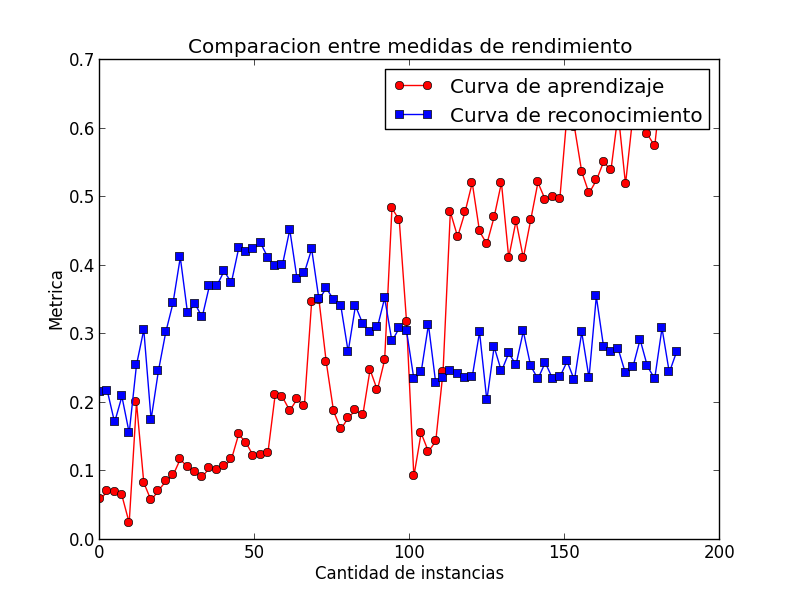
\includegraphics[width=12cm]{curva-apr-vs-rec-dt}
\caption{Curvas de aprendizaje y reconocimiento para el clasificador DT.}
\centering
\end{figure}

El valor las tres medidas en los clasificadores SVM y MNB durante el aprendizaje activo se mantiene constante luego de superar las 10 instancias agregadas al corpus de entrenamiento.

\vspace{3 mm}

\textbf{Conclusión}
Si observaramos aisladamente la medida del \textit{accuracy} para este experimento podría pensarse que todos los clasificadores obtienen resultados significativos, o al menos aceptables. Sin embargo el reconocimiento y el factor kappa ponen en relevancia que los clasificadores MNB y SVM sólo reconocen la clase mayoritaria y etiquetan con ella a todas las instancias.

La figura \ref{curva-apr-vs-rec-dt} con el desempeño en el aprendizaje activo del clasificador DT da indicios de porqué sucede este fenómeno. Si bien el \textit{accuracy} logrado es más bajo, el reconocimiento es más alto en el clasificador final. Analizando las dos curvas de aprendizaje podemos ver que el reconocimiento alcanza su punto máximo con un valor de 0.45 con 60 instancias agregadas al corpus de entrenamiento y posteriormente decae hasta su valor final. Como las primeras instancias agregadas son las de mayor entropía, corresponden a instancias que no pertenecen a la clase mayoritaria. Por lo tanto, formulamos la hipótesis de nuestro experimento número 2 de que entrenar el clasificador con pocas instancias de la clase mayoritaria aumentaría el reconocimiento final.

% [('booksbyauthor', 2), ('listmovies', 1), ('listtvshows', 1), ('howoldis', 1), ('movieduration', 2), ('presidentsof', 1), ('directorof', 2), ('populationof', 2), ('plotof', 2), ('whois', 1), ('whowrote', 2), ('castof', 3), ('whereis', 1), ('moviereleasedate', 2), ('actorsof', 4), ('whereisfrom', 1), ('spokenlanguageof', 2), ('bandmembers', 3), ('showswith', 3), ('musicgenre', 2), ('capitalcityof', 1), ('albumsofband', 4), ('creatorof', 2), ('whatis', 2), ('episodecount', 2), ('actedon', 5), ('bandfoundation', 1), ('moviesbydirector', 3)]
% Testing corpus: 31 recognized instances
% Testing corpus: 186 total instances
% Numbers of classes in Testing corpus  29
% Training corpus 19 recognized questions
% Training corpus total instances  29
% Unlabeled corpus 8 recognized instances
% Unlabeled corpus total instances  505
% booksbyauthor & 3 & 1 & 8 \\
% listmovies & 1 & 1 & 0 \\
% listtvshows & 1 & 1 & 1 \\
% howoldis & 5 & 1 & 14 \\
% movieduration & 1 & 1 & 1 \\
% presidentsof & 2 & 1 & 3 \\
% directorof & 1 & 1 & 0 \\
% populationof & 1 & 1 & 3 \\
% plotof & 1 & 1 & 2 \\
% whois & 1 & 1 & 0 \\
% whowrote & 1 & 1 & 0 \\
% castof & 1 & 1 & 4 \\
% whereis & 3 & 1 & 8 \\
% other & 135 & 1 & 404 \\
% moviereleasedate & 1 & 1 & 1 \\
% actorsof & 2 & 1 & 1 \\
% whereisfrom & 4 & 1 & 8 \\
% spokenlanguageof & 1 & 1 & 3 \\
% bandmembers & 2 & 1 & 6 \\
% showswith & 1 & 1 & 4 \\
% musicgenre & 1 & 1 & 3 \\
% capitalcityof & 1 & 1 & 1 \\
% albumsofband & 5 & 1 & 11 \\
% creatorof & 2 & 1 & 4 \\
% whatis & 1 & 1 & 2 \\
% episodecount & 1 & 1 & 0 \\
% actedon & 4 & 1 & 9 \\
% bandfoundation & 2 & 1 & 2 \\
% moviesbydirector & 1 & 1 & 2 \\

\subsection{Experimento 2}
\vspace{3 mm}
\textbf{Hipótesis} Entrenar el clasificador \textit{MultinomialNB} básico de la librería sklearn con un corpus de entrenamiento con menos cantidad de instancias de clase mayoritaria aumenta el reconocimiento, mientras reduce el \textit{accuracy}.
\vspace{3 mm}

Para realizar este experimento medimos cómo se comporta el \textit{accuracy} y el reconocimiento en función de la cantidad de instacias de clase mayoritaria con que se entrena al clasificador. Es decir, comenzamos con un clasificador entrenado con todas las instancias etiquetadas de clases minoritarias de las que disponemos, 129 en total. Luego agregamos paulatinamente instancias de clase mayoritaria y reentrenamos el clasificador.

Para tener una línea de comparación, también realizamos el mismo proceso con los dos clasificadores utilizados en el experimento anterior.

% Testing corpus: 31 recognized instances
% Testing corpus: 186 total instances
% Numbers of classes in Testing corpus  29
% Training corpus 27 recognized questions
% Training corpus total instances  129
% Unlabeled corpus total instances  405
% booksbyauthor & 3 & 9 & 0 \\
% listmovies & 1 & 1 & 0 \\
% listtvshows & 1 & 2 & 0 \\
% howoldis & 5 & 15 & 0 \\
% movieduration & 1 & 2 & 0 \\
% presidentsof & 2 & 4 & 0 \\
% directorof & 1 & 1 & 0 \\
% populationof & 1 & 4 & 0 \\
% plotof & 1 & 3 & 0 \\
% whois & 1 & 1 & 0 \\
% whowrote & 1 & 1 & 0 \\
% castof & 1 & 5 & 0 \\
% whereis & 3 & 9 & 0 \\
% other & 135 & 0 & 405 \\
% moviereleasedate & 1 & 2 & 0 \\
% actorsof & 2 & 2 & 0 \\
% whereisfrom & 4 & 9 & 0 \\
% spokenlanguageof & 1 & 4 & 0 \\
% bandmembers & 2 & 7 & 0 \\
% showswith & 1 & 5 & 0 \\
% musicgenre & 1 & 4 & 0 \\
% capitalcityof & 1 & 2 & 0 \\
% albumsofband & 5 & 12 & 0 \\
% creatorof & 2 & 5 & 0 \\
% whatis & 1 & 3 & 0 \\
% episodecount & 1 & 1 & 0 \\
% actedon & 4 & 10 & 0 \\
% bandfoundation & 2 & 3 & 0 \\
% moviesbydirector & 1 & 3 & 0 \\

\vspace{3 mm}

\textbf{Resultados} En las siguientes imágenes se muestran los valores del \textit{accuracy} y el reconocimiento para los tres clasificadores \textit{MultinomialNB} (MNB), \textit{Support Vector Machine} (SVM) y \textit{Decision Trees} (DT), utilizando una estrategia de selección de instancias priorizando máxima entropía.

\begin{figure}[h!]\label{curva-apr-hip2}
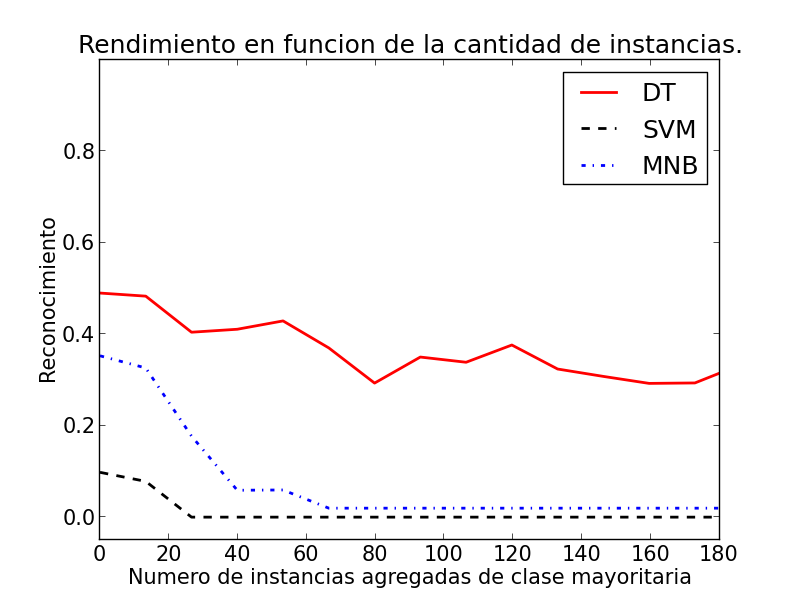
\includegraphics[width=8cm]{recognition-curve-hip2}
% python experiments/grapich_learning_curves.py experiments/results/experiment4/recognitioncurve-full-186-step2-hip2 "DT" experiments/results/experiment5/recognitioncurve-full-186-step2-hip2 "SVM" experiments/results/experiment2/recognitioncurve-full-186-step1-hip2 "MNB"
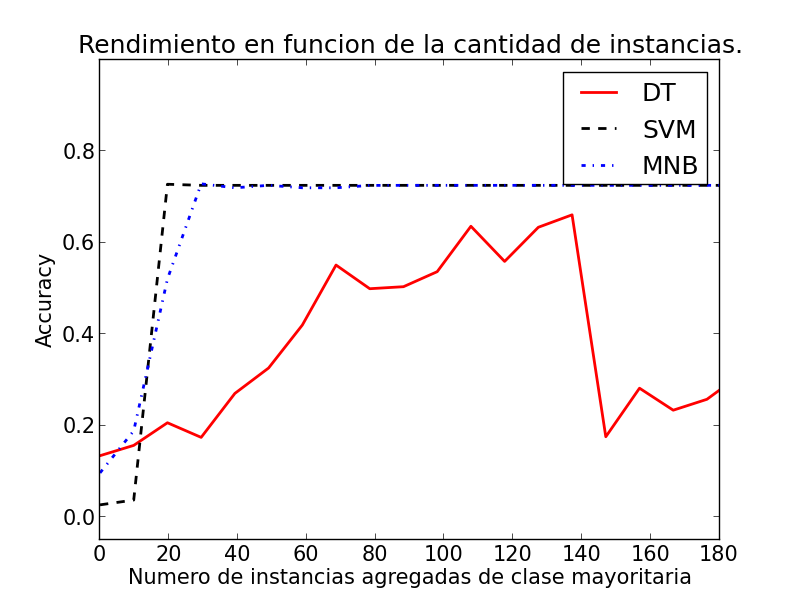
\includegraphics[width=8cm]{learning-curve-hip2}
%python experiments/grapich_learning_curves.py experiments/results/experiment4/learningcurve-full-186-step2-hip2 "DT" experiments/results/experiment5/learningcurve-full-186-step2-hip2 "SVM" experiments/results/experiment2/learningcurve-full-186-step1-hip2 "MNB"
\caption{Curvas de aprendizaje y reconocimiento.}
\centering
\end{figure}

\vspace{3 mm}

\textbf{Conclusión}
Como esperabamos, el reconocimiento es inversamente proporcional a la cantidad de instancias de clase mayoritaria que se utilizan en el entrenamiento. Esto no quiere decir que no deban ser utilizadas, sino que pueden estar abrumando los pocos datos etiquetados de las otras clases que componen el corpus de entrenamiento.

Estos resultados no son extraños en problemas donde se busca reconocer y clasificar una pequeña parte del universo de instancias, como ya hemos visto que plantea \citet{rare-classes-holpedales}. En nuestro caso, estamos clasificando el resto del universo dentro de una clase mayoritaria aunque esto no se corresponda con la realidad. Esta mega-clase engloba las instancias de todas las clases que no podemos reconocer, y como tal no existen características distintivas que permitan al clasificador reconocerlas. Ante tanta diversidad, como podemos observar el desempeño es pobre y se basa sólo en la probabilidad mayor de una etiqueta.


\subsection{Nueva configuración del corpus}

Como resultado del experimento anterior utilizaremos a partir de ahora un corpus no etiquetado (simulado) con la misma cantidad de instancias de la clase mayoritaria que de la segunda clase mayoritaria, es decir, 14 instancias. Si bien esto constituye un corpus muy pequeño, queremos identificar tendencias y no resultados contundentes dado los limitados recursos de los que disponemos.

Al realizar las primeras pruebas tentativas para este corpus notamos que la precisión no podía ser calculada para aquellas clases que se entrenaban con menos de 4 instancias. Esto se debe a que el clasificador no clasifica ninguna instancia como perteneciente a esta clase, lo que resulta en una división por 0 al calcular la métrica. Tengamos en cuenta de que son sólo 4 las instancias que podemos incluir en el corpus de entrenamiento porque previamente seleccionamos 1 o 2 para el corpus de evaluación.

La base de la clasificación es la generalización de la información de los datos de entrenamiento a instancias nunca vistas previamente. La poca cantidad de reformulaciones que pudimos encontrar para estas preguntas conduce a la conclusión de que estas clases no podrán ser discriminadas sin incluir más ejemplos. Por ello tomamos la decisión de excluir estas clases de los siguientes experimentos considerando que no aportan ningún beneficio ni perjuicio a los datos que queremos observar. Se eliminan en este paso 17 clases que representan un 37\% del corpus de entrenamiento y no etiquetado, mientras que sólo es un 10\% del corpus de evaluación.


\subsection{Experimento 3}
\vspace{3 mm}
\textbf{Hipótesis} Las características como las concordancias parciales y los tipos de entidades nombradas son más significativas que las otras para el clasificador \textit{MultinomialNB}.
\vspace{3 mm}

Antes de comenzar con el entrenamiento a través de aprendizaje activo propiamente dicho queremos determinar la configuración de experimentos que maximizará el resultado final. Como mencionamos en el capítulo \ref{capitulo-features}, consideramos que este grupo de características representa mejor a las instancias para esta tarea de categorización en particular. Las preguntas que queremmos analizar tienen una longitud corta y un vocabulario similar, es decir, muchas preguntas contiene palabras como \textit{What}, \textit{Who} o \textit{is}. Sin embargo, estas palabras no son discriminativas de la clase en la mayoría de los casos, sino que dependemos del resto de la frase. Por otro lado, al tener una alta cantidad de clases distintas, es probable que cada una de estas palabras discriminativas esté presente en pocos ejemplos, si no sólo en uno, resultando en un matriz de representación muy esparsa. Por estos motivos suponemos que utilizar derivados simples de las lemmas no formará una frontera de decisión tan clara para el clasificador.

Para probar esta hipótesis entrenamos el clasificador \textit{MultinomialNB} con el corpus de entrenamiento y no etiquetado (simulado) descriptos en la sección anterior preprocesados con distintas combinaciones de características. Compararemos su desempeño en cada una de ellas a través de \textit{accuracy} y reconocimiento. Para un mejor entendimiento de los datos, realizamos un análisis sobre el corpus usado para entrenamiento y obtenemos la distribución de ocurrencias de cada tipo de características en las instancias.

\vspace{3 mm}

\textbf{Resultados} En las siguientes tablas mostramos las mediciones más significativas de \textit{accuracy} y reconocimiento obtenidas sin aprendizaje activo para combinaciones de las siguientes características: Lemmas (L), Bigramas (B), Trigramas (T), Bigramas Mezclados (MB), Etiquetas POS (POS), Entidades nombradas (NE), Tipos de las entidades nombradas (NET) y Concordancia a patrones parciales (PM).

\begin{table}[h!]\label{tabla-exp3}
\centering
\begin{tabular}{l c c}
     & \textit{Accuracy} & Reconocimiento \\ [0.5ex]
    \hline
    L & 0.49 & 0.59 \\ [0.5ex]
    L + B & 0.40 & 0.59 \\ [0.5ex]
    \textbf{L + B + T} & 0.32 & \textbf{0.71} \\[0.5ex]
    L + B + T + MB + POS & 0.30 & 0.59 \\[0.5ex]
    L + B + T + NET + NE & 0.35 & 0.59 \\[0.5ex]
    \textbf{PM} & 0.4 & \textbf{0.65} \\[0.5ex]
    PM + NET & 0.6 & 0.53 \\[0.5ex]
    PM + NET + NE & \textbf{0.64} & 0.43 \\[0.5ex]
    L + PM & 0.43 & 0.59 \\[0.5ex]
    L + B + T + PM & 0.40 & 0.59 \\[0.5ex]
    L + PM + NET & 0.5 & 0.46 \\[0.5ex]
    L + PM + NET + NE + B + T + MB + POS & 0.31 & 0.46 \\[0.5ex]
    \hline
\end{tabular}
\caption{Comparación de desempeño sobre el corpus de evaluación}
\end{table}

En la figura \ref{fig-distribucion-features} cada gráfico de torta ilustra la cantidad de características que ocurren en un número fijo de instancias distribuídas según la clase a la que pertenecen. Es decir, en el primer gráfico la porción de color negro representa cuántos lemmas (L) aparecen sólo en una pregunta de todo el corpus.

\begin{figure}[h!]\label{fig-distribucion-features}
\centering
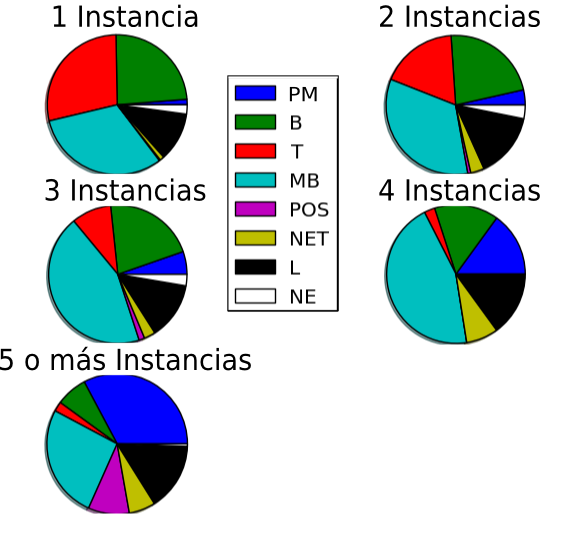
\includegraphics[width=10cm]{clase-feat-inst-labels}
\caption{Distribución de las clases de las características según la cantidad de instancias en las que están presentes.}
\end{figure}

\vspace{3 mm}

\textbf{Conclusión} Primero realizaremos un análisis de los gráficos de torta y luego ahondaremos en el desempeño del clasificador a partir de esa base. Lo primero que notamos es que, como habíamos supuesto, la proporción de Concordancias parciales (PM) y Tipos de entidades nombradas (NET) aumenta mientras aumenta el número de instancias en las que están presentes. Es decir, en proporción hay muchas más reglas que concuerdan con muchas instancias que con una sola. Lo mismo ocurre con las etiquetas POS, pero recordemos que hay pocas de ellas y que en general ocurren muchas veces en el texto. Es decir, en todas las frases hay sustantivos y verbos. Por lo tanto, las consideraremos relevantes. Sin embargo, sí encontramos significativo que la proporción de los lemmas se mantenga constante con respecto a la cantidad de instancias en las que ocurren. Esto nos indica que esta característica podría ser mucho más útil de lo que esperabamos.

El fenómeno contrario ocurre con los Bigramas (B) y Trigramas (T), junto con las Entidades Nombradas en sí (NE), que en general ocurren en pocas instancias dentro del corpus. Por lo tanto, esperaríamos que no se desempeñen bien aisladas sino en conjunto con otras características.

Con respecto al rendimiento del clasificador, ninguna combinación de caraterísticas maximiza tanto el \textit{accuracy} como el reconocimiento. Es decir, que para identificar mejor las instancias de las clases minoritarias es necesario perder precisión sobre la clase mayoritaria. Recordemos que para el fin de nuestra clasificación preferimos lograr un alto reconocimiento.

A partir de la tabla \ref{tabla-exp3} podemos observar claramente que el mayor reconocimiento se obtiene utilizando Concordancias a los patrones (PM) o la combinación Lemmas, Bigramas y Trigramas. Sin embargo, la combinación de estos no arroja buenos resultados. POR QUÉ?

Por otra parte, los Tipos de las entidades nombradas, los Bigramas Mezclados y las Entidades nombradas sólo confunden al clasificador. Si observamos la figura \ref{fig-distribucion-features} estos tipos de características son muy esparsas y ocurren generalemente en menos de tres instancias.

\subsection{Experimento 4}
\vspace{3 mm}
\textbf{Hipótesis} La clasificación obtendrá mejores resultados si se aplica algún método de suavizado como \textit{Tf-idf} o \textit{LSA}.
\vspace{3 mm}

Métodos de suavizado son utilizados comunmente para clasificación de texto y extracción de información para contrarestar la distribución de palabras descripta por la ley de Zipff, donde pocas palabras ocurren muchas veces mientras que la mayoría de los términos están presentes en pocas instancias.

\textit{Tf-idf} hace referencia a Frecuencia de términos y frecuencia inversa de documentos, una medida estadística para determinar cuán importante es una palabra dentro de una instancia o documento. Se calcula como el producto de otras dos medidas: la Frecuencia del término es la cantidad de veces que el término ocurre en la instancia, y la Frecuencia inversa del documento que cuenta inversa de la cantidad de veces que el término aparece en todo el corpus. Como resultado, palabras que ocurren pocas veces en el corpus y se concentran sólo en una porción de instancias toman más relevancia con respecto a palabras que ocurren en muchas intancias, ya que se consideran más representativas de la instancia. Ha sido utilizado por \citet{tackling-mnb} como una forma de modelado alternativa para el clasificador Bayesiano ingénuo.

\textit{LSA} o Análisis de semántica latente es una técnica introducida por \citet{lsa} para superar los problemas de utilizar aproximaciones basadas sólo en términos para el procesamiento de lenguaje natural. Supone que existe una estructura semántica oculta por la aleatoriedad del vocabulario e intenta minimizar el ruido a través de técnicas estadísticas. \textit{LSA} utiliza una técnica llamada Descomposición en valores singulares o \textit{SVD} que descompone la matriz de representación en un nuevo espacio vectorial de forma que se reduce la dimensionalidad (tiene menos características) mientras se preserva la relación entre las las características restantes y las instancias.

Para aplicar estos dos métodos usamos las clases \textit{TfidfTransformer} y \textit{TruncatedSVD} de la librería \textit{scikit-learn}. Luego de preprocesar todos los corpus con estos métodos entrenamos el clasificador \textit{MultinomialNB} y comprobamos su rendimiento sobre el corpus de evaluación.

\vspace{3 mm}

\textbf{Resultados} En la siguiente tabla mostramos las mediciones más significativas de \textit{accuracy} y reconocimiento obtenidas sin aprendizaje activo para combinaciones de las siguientes características: Lemmas (L), Bigramas (B), Trigramas (T), Bigramas Mezclados (MB), Etiquetas POS (POS), Entidades nombradas (NE), Tipos de las entidades nombradas (NET) y Concordancia a patrones parciales (PM), aplicando métodos de suavizado de Tf-idf y LSA.

\begin{table}[h]\label{tabla-exp3}
\centering
\begin{tabular}{l c c | c c}
     & \multicolumn{2}{c|}{Tf-Idf} & \multicolumn{2}{c}{LSA}\\ [0.5ex]
     & \textit{Accuracy} & Reconocimiento & \textit{Accuracy} & Reconocimiento \\ [0.5ex]
    \hline
    L & 0.45 & 0.4 & 0.72 & 0.37 \\[0.5ex]
    L + B + T & 0.36 & 0.34 & 0.74 & 0.43 \\[0.5ex]
    PM & 0.44 & \textbf{0.59} & 0.41 & 0.43 \\[0.5ex]
    \textbf{PM + L} & 0.35 & 0.5 & 0.44 & \textbf{0.68} \\[0.5ex]
    PM + L + LNT & 0.50 & 0.50 & 0.79 & 0.25\\[0.5ex]
    \textbf{PM + L + B + T} & 0.32 & 0.46 & 0.49 & \textbf{0.68} \\[0.5ex]
    PM + L + B + T + LNT & 0.40 & 0.43 & 0.79 & 0.31 \\[0.5ex]
    PM + LTN + LN & \textbf{0.64} & 0.43 & 0.74 & 0.09 \\[0.5ex]
    PM + LTN + LN + L & 0.52 & 0.46 & \textbf{0.76} & 0.21 \\[0.5ex]
    Todos & 0.32 & 0.4 & 0.67 & 0.53 \\[0.5ex]
    \hline
\end{tabular}
\caption{Comparación de desempeño sobre el corpus de evaluación con distintas caraterísticas y técnicas de suavizamiento.}
\end{table}
% L + PM + NET + NE + B + T + MB + POS
No incluímos los resultados de los experimentos utilizando ambos métodos ya que ninguno de ellos dió mejores resultados que los mencionados anteriormente.

Los datos expresados con el preprocesamiento de LSA tienen el número de dimensiones que maximizan el resultado. Para las combinaciones PM + L + B + T y PM + L se utilizaron 250 características.

En la tabla \ref{prec-recall-mejor-solucion} se muestra la precisión y la exhaustividad para cada una de las clases utilizando las dos mejores combinaciones de características de la tabla \ref{tabla-exp3}. En la última columna se incluye el número de instancias para cada clase dentro del corpus de evaluación.

\begin{table}[h]\label{prec-recall-mejor-solucion}
\centering
\begin{tabular}{l c c | c c | c}
     & \multicolumn{2}{c|}{PM + L + B + T + LSA} & \multicolumn{2}{c}{PM + L + LSA} &\\ [0.5ex]
    Clase & Precisión & Exhaustividad & Precisión & Exhaustividad & Instancias\\ [0.5ex]
    \hline
    actedon & 0.57 & 1.00 & 0.57 & 1.00 & 4\\ [0.5ex]
    \textbf{albumsofband} & 0.33 & 0.80 & \textbf{0.36} & \textbf{0.86} & 5\\ [0.5ex]
    bandmembers & 1.00 & 0.50 & 1.00 & 0.50 & 2\\ [0.5ex]
    \textbf{booksbyauthor} & \textbf{1.00} & 0.67 & 0.50 & 0.67 & 3\\ [0.5ex]
    castof & 0.00 & 0.00 & 0.00 & 0.00 & 1\\ [0.5ex]
    \textbf{creatorof} & \textbf{0.17} & 1.00 & 0.15 & 1.00 & 2\\ [0.5ex]
    \textbf{howoldis} & \textbf{0.09} & 1.00 & 0.08 & 1.00 & 5\\ [0.5ex]
    \textbf{other} & 0.92 & 0.44 & \textbf{0.93} & 0.38 & 135\\ [0.5ex]
    presidentsof & 0.50 & 0.50 & 0.50 & 0.50 & 2\\ [0.5ex]
    showswith & 0.00 & 0.00 & 0.00 & 0.00 & 1\\ [0.5ex]
    \textbf{whereis} & \textbf{0.38} & 1.00 & 0.33 & 1.00 & 3\\ [0.5ex]
    whereisfrom & 0.00 & 0.00 & 0.00 & 0.00 & 4\\ [0.5ex]
    & & & & & \\
    Promedio/total & \textbf{0.82} & \textbf{0.49} & 0.81 & 0.44 & 167\\ [0.5ex]
    \hline
\end{tabular}
\caption{Comparación de desempeño sobre el corpus de evaluación con distintas caraterísticas y técnicas de suavizamiento.}
\end{table}


\vspace{3 mm}

\textbf{Conclusión}
Cómo explico por qué el tdidf no funciona si en la mayoría de los casos anda bien???

Podemos observar que, como esperabamos, agregar \textit{LSA} permite combinar mejor los Lemmas, Bigramas y Trigramas con las Concordancias a patrones. Aún sin esta combinación no alcanza los valores de reconocimiento que pudimos observar en el experimento anterior, aumenta significativamente el \textit{accuracy}. Vemos que este en un fenómeno general de todas las combinaciones, por lo que esperamos que con un corpus mayor esta técnica permita aumentar el rendimiento sobre todas las clases.

Un resultado sorprendente es el bajo reconocimiento de la combinación L + B + T con LSA, que en el experimento anterior obtuvo los mejores resultados. Un fenómeno común que observamos al reducir la dimensionalidad es que la clase mayoritaria vuelve a adquirir un gran peso. Por ello aumenta tanto el \textit{accuracy} de todas las combinaciones.

La tabla \ref{prec-recall-mejor-solucion} indica, con un análisis más detallado, que la mejor combinación de características es L + B + T + PM + LSA.

\subsection{Experimento 5}\label{experimento-aa-instancias}
\vspace{3 mm}
\textbf{Hipótesis} El aprendizaje activo sobre instancias permite al clasificador obtener el mismo rendimiento con menor cantidad de instancias.
\vspace{3 mm}

En este experimento simulamos la interacción con un usuario como describimos en la sección \ref{descripcion-corpus}, comenzando con un corpus de entrenamiento pequeño el ciclo de aprendizaje activo. El aprendedor selecciona la siguiente instancia de un corpus etiquetado (sin conocer la verdadera clase) para enviar al oráculo, pero en lugar de interactuar con un usuario obtenemos las respuestas del mismo corpus.

Para esta sección decidimos preprocesar los datos utilizando Lemmas, Bigramas, Trigramas y Concordancias a patrones y aplicando LSA, basándonos en los resultados del experimento anterior. Evaluaremos la curva de aprendizaje para el \textit{accuracy} y para el reconocimiento con tres estrategias de selección de instancias distintas: al azar, con mayor entropía y con menor entropía. El clasificador utilizado es \textit{MultinomialNB} junto con el módulo ActivePipeline.

Recordemos que las instancias con menor entropía son aquellas sobre las que el clasificador tiene mayor seguridad, y por lo tanto aportan menos información. Seleccionar instancias con menor entropía primero permitirá al clasificador asegurar la información que se asume es verdadera. Consideramos que esta es una buena estrategia teniendo en cuenta la reducida cantidad de ejemplos con los que comienza el entrenamiento del clasificador.

El clasificador se reentrenó y se aplicó un ciclo del algoritmo Esperanza-Maximización luego de agregar una instancia al corpus de entrenamiento.


\begin{figure}[h!]\label{fig-aa-comparision}
\centering
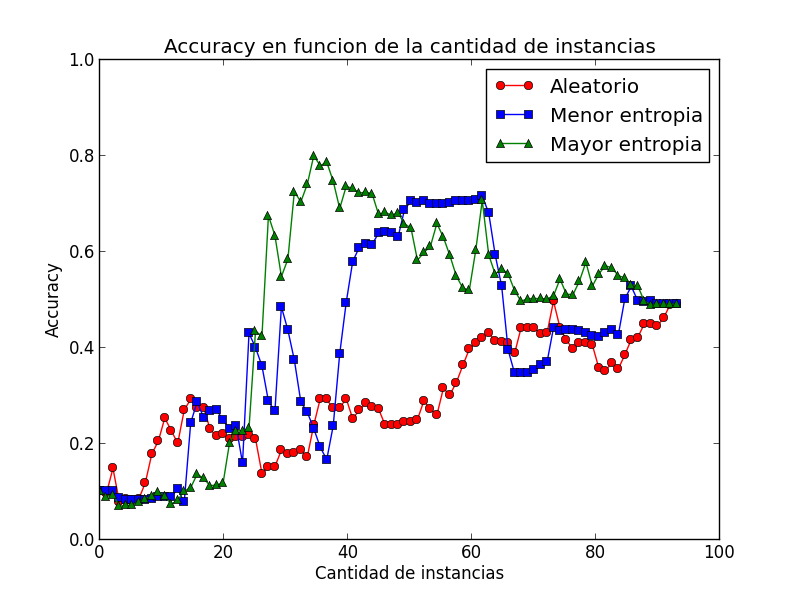
\includegraphics[width=10cm]{learningcurve-aa-exp5}
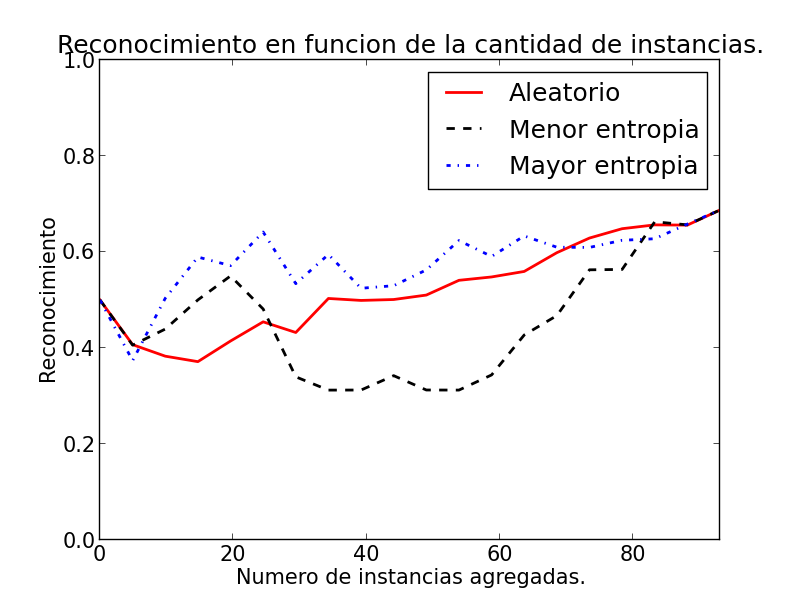
\includegraphics[width=10cm]{recognitioncurve-aa-exp5}
\caption{Desempeño del clasificador con aprendizaje activo y distintas estrategias de selección de instancias.}
\end{figure}
\vspace{3 mm}

\textbf{Resultados} En la figura \ref{fig-aa-comparision} mostramos la evolución del \textit{accuracy} y del reconocimiento para las tres estrategias de selección de instancias: aleatoria, mayor entropía y menor entropía.


\vspace{3 mm}

\textbf{Conclusión}

Como podemos observar en la curva de aprendizaje ambas estrategias se desempeñan mejor que un aprendizaje aleatorio. Sin embargo, la selección por mayor entropía maximiza tanto el \textit{accuracy} como el reconocimiento.

Y qué más puedo decir????!!!!

\subsection{Corpus de características}

% Los (siguientes) experimentos que solicitan al oráculo información sobre instancias y características se realizaron alternando pocas preguntas relativas a instancias y la misma cantidad relativas a características. Si bien los dos ciclos de etiquetado son completamente independientes en el sistema, tomamos esta desición para eliminar las diferencias entre experimentos que puedan introducirse a partir de la elección de los usuarios. Otra punto en el que difieren nuestros experimentos de una sesión no simulada con un usuario es la cantidad de veces que se reentrena. Con objeto de obtener una medición precisa de la curva de aprendizaje reentrenamos el clasificador luego de cada ronda intancias-características descriptas anteriormente. Esto es costoso para grandes volúmenes de datos y podría hacer perder al sistema su interactividad.

% Para poder realizar experimentos automáticos sin que el usuario tenga que ingresar la misma información repretidas veces decidimos guardar las respuestas obtenidas. Por ello agregamos etiquetas al corpus no etiquetados, que por supuesto no son consultadas, y creamos un corpus de asociaciones características-clases.

Antes de comenzar con estos experimentos utilizamos el módulo \textit{ActivePipeline} para etiquetar manualmente características. El corpus de características no es más que una matriz ternaria con tres valores posibles: asociación positiva, no asociación, desconocido. De esta forma también alamcenamos información para evitar preguntar a un usuario por las características que ya han sido vistas pero no están relacionadas a esa clase en particular. Observemos que esta forma de guardar la información soporta etiquetas de múltiples clases para una misma característica.

Todas las instancias etiquetadas fueron preprocesadas utilizando como características las concordancias a patrones, lemmas, bigramas y trigras. La cantidad total de características extraídas es 3781, incluyendo todos los corpus. No se utilizó la técnica de LSA aunque había arrojado buenos resultados ya que afecta la dimensionalidad del modelo y por lo tanto el mapeo entre las columnas de la matriz de representación y las características seleccionadas.

Para la creación del corpus de características se realizó una sesión de aproximadamente una hora utilizando un clasificador \textit{MultinomialNB} entrenado con el corpus de entrenamiento y el corpus no etiquetado (simulado). Para elegir las características a ser etiquetadas se las ordenó por mayor coocurrencia con la clase y por mayor ganancia de información.

De las 2891 características que se presentaron al usuario, éste etiquetó como asociaciones positivas 355. En la tabla \ref{dist-feat-corpus} se muestra la distribución de características asociadas a cada clase.

\begin{table}[h]\label{dist-feat-corpus}
\centering
\begin{tabular}{l c}
    Clase & Características asociadas\\ [0.5ex]
    \hline
    actedon & 40 \\ [0.5ex]
    albumsofband & 43 \\ [0.5ex]
    bandmembers &  23 \\ [0.5ex]
    booksbyauthor &  42 \\ [0.5ex]
    castof & 42 \\ [0.5ex]
    creatorof & 16 \\ [0.5ex]
    howoldis & 45 \\ [0.5ex]
    other & 0 \\ [0.5ex]
    presidentsof & 20 \\ [0.5ex]
    showswith & 30 \\ [0.5ex]
    whereis & 26 \\ [0.5ex]
    \hline
\end{tabular}
\caption{Distribución de la cantidad de etiquetas de características para cada una de las clases}
\end{table}

No se realizaron etiquetamientos sobre la clase \textit{other} ya que, al no constituir una clase semántica propiamente dicha, no hay características que indiquen que una pregunta pertenece a esa clase.

Cabe destacar que en todos los experimentos siguientes hemos utilizado este corpus para el entrenamiento con características.

\subsection{Experimento 6}
\vspace{3 mm}
\textbf{Hipótesis} Entrenar el clasificador utilizando información sobre las características incrementará su rendimiento.
\vspace{3 mm}

Nuestro objetivo principal es medir el aumento del rendimiento de un clasificador \textit{FeatMultinomialNB} entrenado solamente con instancias y entrenado con instancias y características. Adicionalmente queremos analizar cómo varía este resultado de acuerdo a la cantidad de instancias utilizadas para el entrenamiento. Es posible que el impacto del corpus de características disminuya al agregar instancias.

Un parámetro muy importante para esta tarea es el peso adicional de las características llamado $\alpha$ en la ecuación \ref{eq-feat-boost}. Este peso adicional será sumado directamente a la matriz de probabilidad $\hat{P}(f_k|c_j)$ si la característica $f_k$ ha sido asociada a la clase $c_j$. \citet{dualist} demuestra en sus experimentos que cualquier valor entre 0.5 y 100 para este parámetro es indistinto, pero probaremos si esta hipótesis es válida para nuestra configuración también.

El primer experimento a realizar será entrenar el clasificador con el corpus de entrenamiento que tiene una instancia por clase y el corpus de features descripto anteriormente con distinto pesos adicionales. Realizaremos el mismo trabajo con entrenando con todo el conjunto de instancias anotadas y finalmente compararemos los resultados.

\vspace{3 mm}

\textbf{Resultados}

En la figura \ref{comp-feature-boost} se comparan las tres medidas de desempeño del clasificador utilizando distintos pesos adicionales. Se comparan dichas medidas entre un clasificador que utiliza sólo el corpus de entrenamiento con 12 instancias y un clasificador que utiliza además el corpus no etiquetado (simulado).

\begin{figure}[h!]\label{comp-feature-boost}
\centering
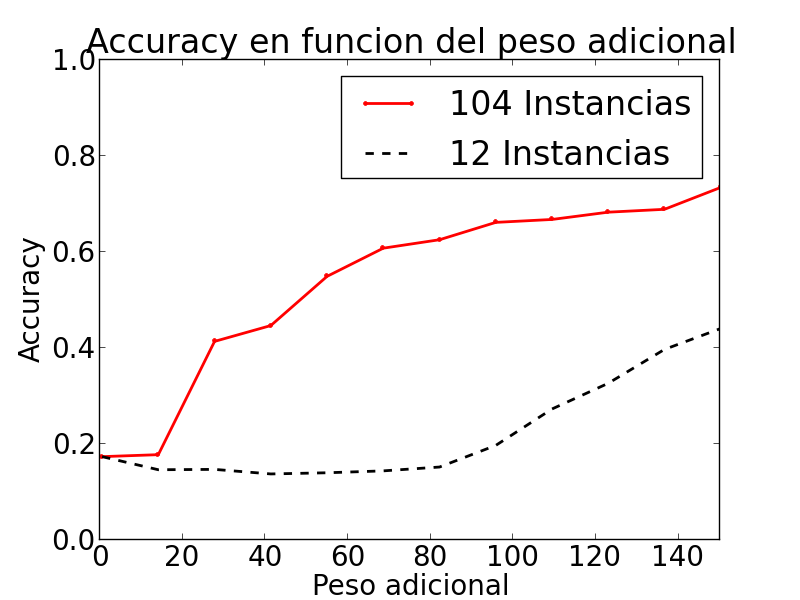
\includegraphics[width=6cm]{accuracy-vs-feat-boost-2corpus}
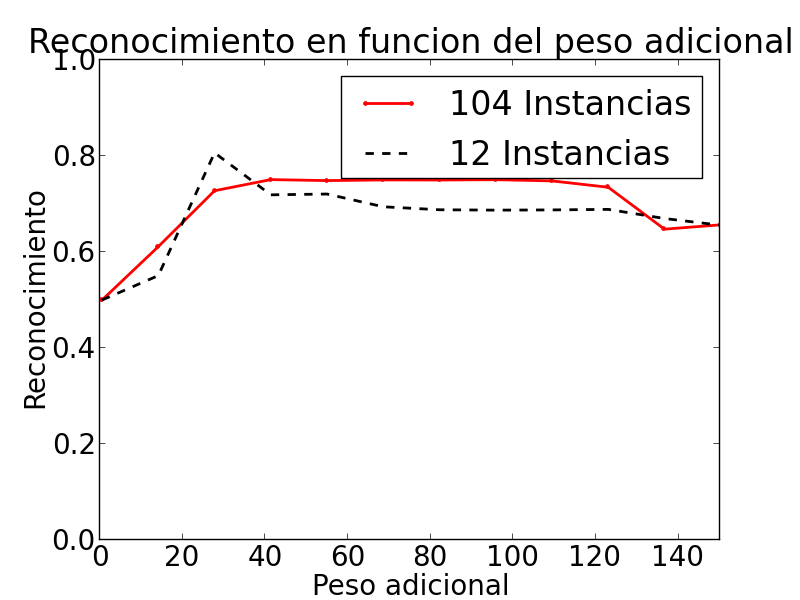
\includegraphics[width=6cm]{recog-vs-feat-boost-2corpus}
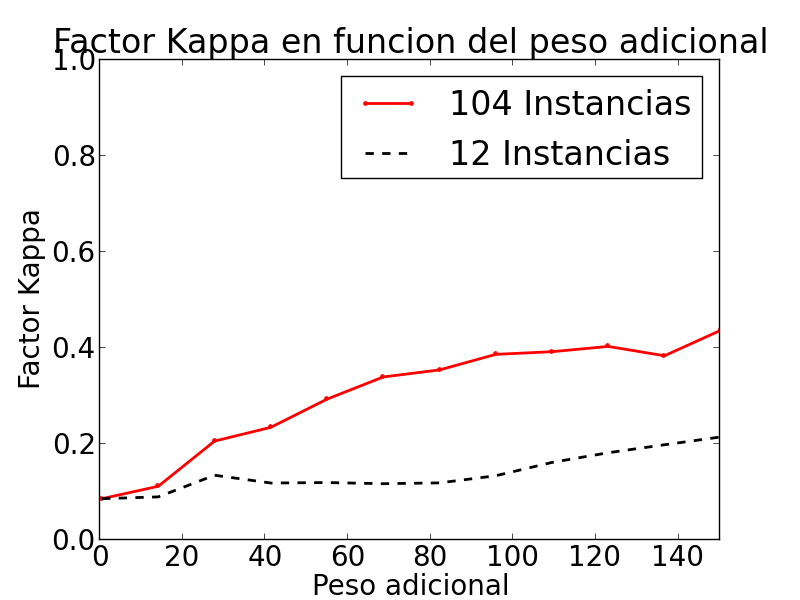
\includegraphics[width=6cm]{kappa-vs-feat-boost-2corpus}
\caption{Rendimiento del clasificador entrenado con características para distintos pesos adicionales sobre dos corpus.}
\end{figure}

En la figura \ref{comp-feat-tr-inst} se muestra el \textit{accuracy} y reconocimiento para el clasificador entrenado con y sin características, utilizando distintas cantidades de instancias.

\begin{figure}[h!]\label{comp-feat-tr-inst}
\centering
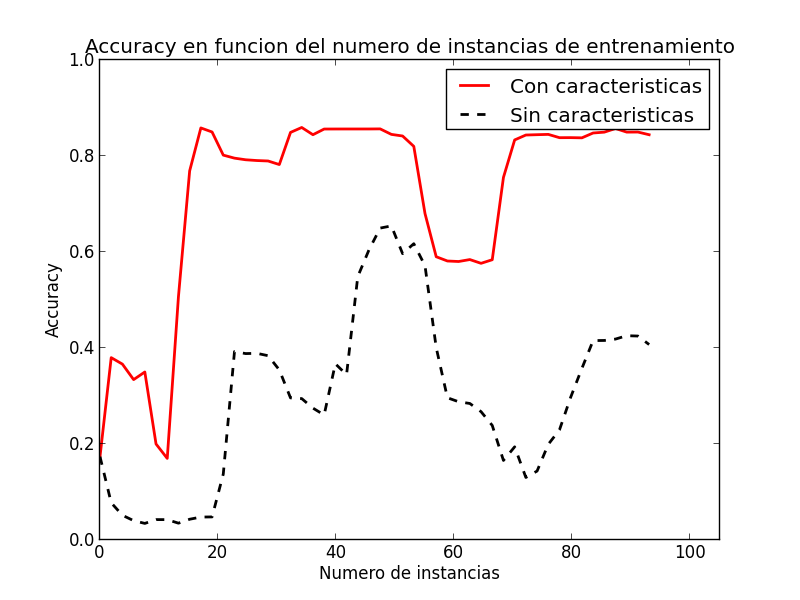
\includegraphics[width=7cm]{accuracy-vs-instancia-feat}
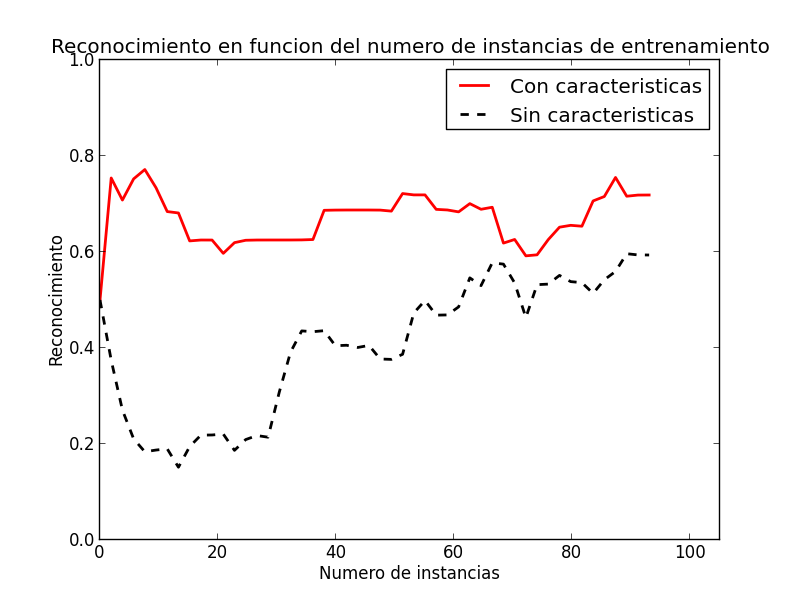
\includegraphics[width=7cm]{recog-vs-instancia-feat}
\caption{Rendimiento del clasificador entrenado con características con un peso adicional de 100 sobre distintas cantidades de instancias.}
\end{figure}
\vspace{3 mm}

\textbf{Conclusión}

El entrenamiento con características obtuvo el mismo reconocimiento en ambos corpus.
No tiene efecto en el accuracy porque no hay etiquetas de la clase otro.
El boost no varía (tanto) para el reconocimiento (como decía \citet{dualist}) pero sí para el accuracy.
Los resultados son extremos porque el corpus que estamos utilizando es extremo.
El aprendizaje activo es una buena opción si conseguir instancias es muy dificultoso, ya que en cualquier conjunto de preguntas aleatorio el usuario estaría todo el tiempo etiquetando instancias que no son relevantes.


\subsection{Experimento 7}
\vspace{3 mm}
\textbf{Hipótesis} El aprendizaje activo sobre características permite al clasificador aprender más rápidamente.
\vspace{3 mm}

Al igual que en el experimento \ref{experimento-aa-instancias}, compararemos estrategias inteligentes de selección de características para agregar al corpus contra selección aleatoria.

Como propusimos en la sección \ref{instance-selection} utilizaremos la ganancia de información de cada característica como estrategia de selección. Realizaremos experimentos asignando mayor relevancia a mayor ganancia de información y viceversa.

Por qué tiene sentido hacer IG al revés?

Siguiendo los experimentos ateriores utilizaremos el clasificador \textit{FeatMultinomialNB} con un peso adicional de 100 para las características etiquetadas. Como no estamos interactuando con un usuario, no necesitamos decidir primero sobre que clase etiquetaremos sino simplemente agregaremos al conjunto de entrenamiento la característica seleccionada por la estrategia con todas las clases con las que esté asociada.

Inicialmente vamos a utilizar el clasificador entrenado con todas las instancias para medir correctamente tanto el \textit{accuracy} como el reconocimiento.

\vspace{3 mm}

\textbf{Resultados}

\begin{figure}[h!]\label{comp-feat-selection}
\centering
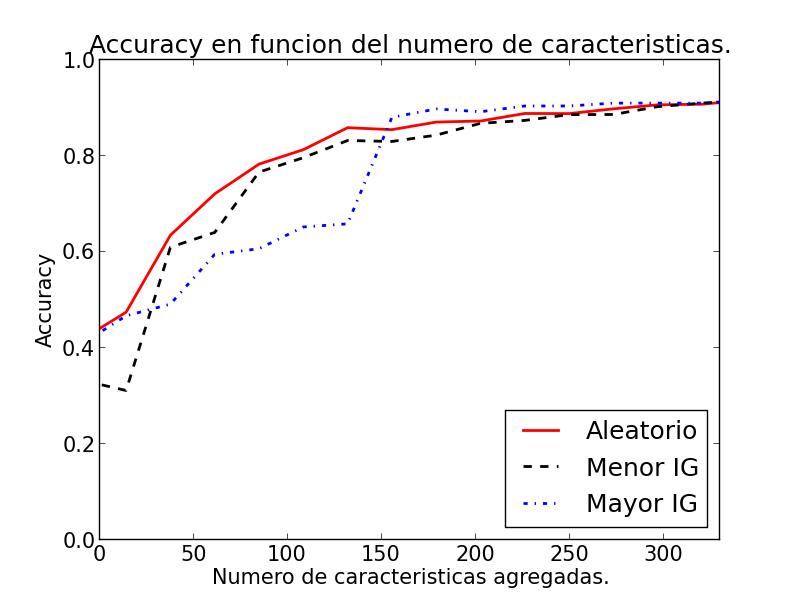
\includegraphics[width=8cm]{learningcurve-aa-feat}
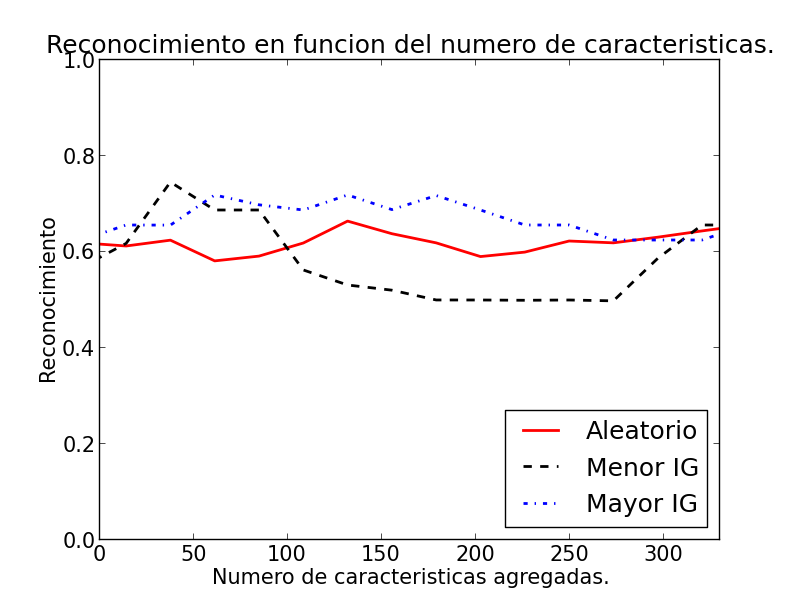
\includegraphics[width=8cm]{recognitioncurve-aa-feat}
\caption{Curvas de aprendizaje del clasificador entrenado con características con un peso adicional de 100.}
\end{figure}
\vspace{3 mm}

tomamos 5 promedios


% \subsection{Hipótesis 2}
% \textbf{El aprendizaje activo sobre instancias y características obtiene mejores resultados que el aprendizaje activo sobre instancias o características por separado.}

% \subsection{Experimento 4}
% \textbf{Hipótesis} ??.

% \subsection{Experimento 5}
% \textbf{Hipótesis} Seleccionar features para etiquetar que tengan alta confiabilidad/correlación, y luego de superado un cierto límite pasar a los que tiene baja confiabilidad/correlación permite al clasificador eliminar el ruido no introducido por la baja cantidad de ejemplos y al mismo tiempo expandir la cobertura.
% Dejar para mas adelante

% Experimento 6
% Information gain sobre todo el corpus o solo el etiquetado.
% IG sobre el corpus anotado + frecuencia en no anotado vs IG sobre todo el corpus anotado y no anotado.

% Experimento 7
% Coocurrencia de features con otros features. (Información mutua)
% Un feature se rankea mas alto si coocurre con features que se rankean alto. Tomando como base la frecuencia.

% Experimento 8
% Information gain sirve o alcanza sólo con usar coocurrencia? Para esto podemos ver la posicion de los features que elige el usuario.

\include{resultados}
\include{conclusiones}

%now enable appendix numbering format and include any appendices
%\appendix
\include{apendice}
%\include{appendix2}

%next line adds the Bibliography to the contents page
\addcontentsline{toc}{chapter}{Bibliography}
%uncomment next line to change bibliography name to references
%\renewcommand{\bibname}{References}
\bibliography{biblio}        %use a bibtex bibliography file refs.bib
\bibliographystyle{plainnat}

\end{document}

